\documentclass[11pt]{article}
\usepackage[a4paper,margin=19mm,headheight=15pt]{geometry}
\usepackage[T1]{fontenc}
\usepackage{lmodern,microtype,amsmath,amssymb,mathtools,array,longtable,booktabs,enumitem}
\usepackage[most]{tcolorbox}
\usepackage{fancyhdr,hyperref,bookmark,needspace,titlesec}
\usepackage{tikz}
\definecolor{navy}{HTML}{183650}
\definecolor{teal}{HTML}{007D83}
\definecolor{amber}{HTML}{A65F08}
\definecolor{plum}{HTML}{6B3A7A}
\definecolor{crimson}{HTML}{A3243A}
\hypersetup{colorlinks=true,linkcolor=teal,urlcolor=teal}
\pagestyle{fancy}\fancyhf{}
\fancyhead[L]{\small MATH6310 | Metric Spaces \& Topology: step-by-step exam revision}
\fancyhead[R]{\small Sai Vanam}\fancyfoot[C]{\thepage}
\setlength{\parindent}{0pt}\setlength{\parskip}{5pt}
\setlist{nosep,leftmargin=*}
\linespread{1.1}
\tcbset{enhanced,breakable,colback=blue!2!white,colframe=navy,boxrule=.6pt,arc=1.5mm,
  left=3mm,right=3mm,top=2mm,bottom=2mm,before skip=8pt,after skip=8pt,fonttitle=\bfseries}
\newtcolorbox{defn}[1]{title={Definition: #1}}
\newtcolorbox{thm}[1]{title={Theorem: #1},colframe=plum,colback=plum!3!white}
\newtcolorbox{plain}{title={In plain words},colframe=black!45,colback=black!2!white}
\newtcolorbox{steps}[1]{title={Step by step: #1},colframe=teal,colback=teal!3!white}
\newtcolorbox{example}[1]{title={Worked example: #1},colframe=navy!70,colback=white}
\newtcolorbox{exam}[1]{title={Exam-style question: #1},colframe=amber,colback=yellow!5!white}
\newtcolorbox{answer}{title={Model answer},colframe=teal,colback=green!2!white}
\newtcolorbox{tip}{title={Exam tips and common mistakes},colframe=crimson,colback=red!2!white}
\newtcolorbox{note}[1]{title={#1}}
\newcommand{\R}{\mathbb R}\newcommand{\Q}{\mathbb Q}\newcommand{\N}{\mathbb N}
\newcommand{\Z}{\mathbb Z}\newcommand{\C}{\mathbb C}
\newcommand{\cl}[1]{\overline{#1}}
\newcommand{\inte}{\operatorname{Int}}\newcommand{\diam}{\operatorname{diam}}
\newcommand{\dist}{\operatorname{dist}}\newcommand{\Lip}{\operatorname{Lip}}
\newcommand{\Ran}{\operatorname{Ran}}\newcommand{\id}{\operatorname{id}}
\newcommand{\dsup}{d_{\sup}}
\newcommand{\norm}[1]{\left\lVert#1\right\rVert}
\newcommand{\oi}[2]{\mathopen{]}#1,#2\mathclose{[}}   % open interval ]a,b[
\newcommand{\lo}[2]{\mathopen{[}#1,#2\mathclose{[}}   % [a,b[
\newcommand{\ro}[2]{\mathopen{]}#1,#2\mathclose{]}}   % ]a,b]
\newcommand{\cpl}{^{\complement}}
\renewcommand{\thesection}{\arabic{section}}
\titleformat{\section}{\Large\bfseries\color{navy}}{Part \thesection}{1em}{}
\titleformat{\subsection}{\large\bfseries\color{navy}}{\thesubsection}{0.8em}{}
\newcommand{\topic}[1]{\par\Needspace{40mm}\subsection{#1}}
\setcounter{tocdepth}{2}

\begin{document}
\begin{titlepage}
\vspace*{14mm}
{\Huge\bfseries\color{navy} Metric Spaces \& Topology\par}
\vspace{4mm}
{\LARGE MATH6310: step-by-step exam revision guide\par}
\vspace{6mm}
{\large The whole module (Sections 0--6), written to be followed one step at a time\par}
\vspace{2mm}{\large Prepared for Sai Vanam, 2026/27\par}
\vspace{10mm}
\begin{note}{What is in this guide}
\begin{itemize}
\item \textbf{Part 0}: how the exam works, how to write a proof that earns marks, and ten
  proof templates that cover almost every question.
\item \textbf{Parts 1--5}: every topic in lecture order. Each topic gives the definition, what it
  means in plain words, a step-by-step method, worked examples, exam-style questions with model
  answers, and common mistakes.
\item \textbf{Part 6}: an exam question bank in the style of the 2022--2025 MATH316 papers,
  sorted from easy to hard, with full model answers.
\item \textbf{Part 7}: a full mock paper with worked solutions.
\item \textbf{Part 8}: quick-reference sheets: definitions, theorems with their hypotheses,
  a counterexample bank, and a ``which tool do I use?'' table.
\end{itemize}
\end{note}
\begin{note}{Sources and how far to trust them}
The official lecture notes \emph{MS+T Sections 0--6} (last edited 7 September 2026) are the
authority, and this guide uses their notation: $B_r(a)$, $B_r[a]$, $\inte A$, $\cl A$,
$\partial A$, $\dist_A$, $\diam$, $\Lip$, $\ell^p(N)$, $\ell^\infty(S;E)$, $\oi ab$ for open
intervals. The exam-style questions follow the topics of the 2022--2025 MATH316 papers as listed
in your earlier guides. Those papers do not guarantee what this year's paper will ask.
Every solution here has been worked out again from the lecture notes.
Items the notes mark \textbf{non-examinable} are labelled as such.
\end{note}
\begin{note}{How to use the coloured boxes}
\textbf{Blue}: definitions. \textbf{Purple}: theorems. \textbf{Grey}: the idea in plain words.
\textbf{Teal}: step-by-step methods and model answers. \textbf{Gold}: exam-style questions (try
them before reading the answer). \textbf{Red}: mistakes that lose marks.
\end{note}
\vfill
{\small Recommended order: read Part 0, then one Part per session, doing every gold question
yourself first. In the final week, do Part 7 under timed conditions and learn Part 8 by heart.}
\end{titlepage}
\tableofcontents\clearpage

\setcounter{section}{-1}
\section{How to answer exam questions in this module}

\topic{The big picture: what the module is about}
The whole module is built from one idea: a \emph{distance function} $d$ on a set $S$ obeying
three rules (the metric axioms). From those three rules alone we rebuild everything you know
from real analysis:

\begin{center}
\begin{tabular}{@{}lll@{}}
\toprule
Real analysis idea & Metric space version & Where \\ \midrule
$|x-y|$ & $d(x,y)$ & Section 0, 3 \\
$\oi{a-r}{a+r}$ & open ball $B_r(a)=\{x: d(x,a)<r\}$ & Section 3 \\
$x_n\to a$ & $d(x_n,a)\to 0$ & Section 3 \\
open interval, closed interval & open set, closed set & Section 4 \\
$\varepsilon$--$\delta$ continuity & continuity, preimages of open sets are open & Section 4 \\
Cauchy sequences converge in $\R$ & complete metric space & Section 5 \\
Bolzano--Weierstrass & sequentially compact set & Section 6 \\
\bottomrule
\end{tabular}
\end{center}

Sections 1 and 2 are the toolkit (sets, functions, countability, sup/inf, sequences, norms).
They are partly revision, but they supply the tools for the main proofs.

\begin{plain}
Almost every exam question is one of three kinds:
\begin{enumerate}
\item \textbf{Define / state}: write down a definition or theorem exactly.
\item \textbf{Prove}: show that something has a property (is a metric, is open, is complete,
  is compact, is continuous, \dots). There is a template for each one, given below.
\item \textbf{Disprove / give an example}: show that something can fail. You need a
  counterexample, and you must \emph{check} that it works. Part 8 has a counterexample bank.
\end{enumerate}
\end{plain}

\topic{What the past papers looked like}
The 2022--2025 papers (code MATH316) had four or five long questions, each split into parts
worth a few marks to about ten marks. The recurring topics were:
\begin{itemize}
\item metric axioms, triangle-inequality estimates, discrete metric, isometries into $\R^2$;
\item open/closed sets, interior, closure, metric subspaces (relatively open sets);
\item continuity via preimages; density; separability;
\item equivalent metrics ($\min\{d,1\}$, $d/(1+d)$, $\arctan$); product metrics;
\item completeness: closed subsets of complete spaces, $\ell^\infty(S;E)$, $C_b(E;E')$;
\item Banach's Contraction Mapping Theorem;
\item sequential compactness: continuous images, closed subsets, products, Heine--Borel,
  and counterexamples.
\end{itemize}
The parts usually go in the order \emph{define} $\to$ \emph{easy proof} $\to$
\emph{example/counterexample} $\to$ \emph{harder proof}. Marks for definitions are the easiest
marks on the paper, so learn them word for word (Part 8.1).

\topic{How to write a proof that earns full marks}
\begin{steps}{writing any proof}
\begin{enumerate}
\item \textbf{Write down what you are given} in symbols. (``Let $(x_n)$ be a Cauchy sequence
  in $E$.'')
\item \textbf{Write down what you must show}, using the definition. (``We must find $a\in E$
  with $d(x_n,a)\to 0$.'') This one line often earns a mark by itself and tells you what to
  do next.
\item \textbf{Choose the template} (below) that matches the goal.
\item \textbf{Work through it}, quoting a reason for every inequality: ``by the triangle
  inequality (MS3)'', ``since $U$ is open'', ``by completeness of $E$''.
\item \textbf{When you use a theorem, check its hypotheses aloud}: ``$E$ is complete and
  $\phi$ is a strict contraction, so by Banach's CMT\dots''.
\item \textbf{Finish with a conclusion sentence} that repeats the claim.
\end{enumerate}
\end{steps}

\begin{tip}
\begin{itemize}
\item Fix the order of quantifiers: ``$\forall \varepsilon>0\ \exists N$'' means $N$ may depend
  on $\varepsilon$; ``$\exists \delta\ \forall x$'' (uniform) means one $\delta$ works for all
  $x$.
\item Strict inequalities can become non-strict in a limit: if $d(x_n,a)<r$ for all $n$ and
  $x_n\to p$, you only get $d(p,a)\le r$.
\item ``Not open'' does \emph{not} mean ``closed''. Most sets are neither.
\item An example never proves a ``for all'' statement, but one counterexample disproves it.
\item When giving a counterexample, verify \emph{both} that the hypotheses hold \emph{and}
  that the conclusion fails.
\end{itemize}
\end{tip}

\topic{The ten proof templates}
Learn these. Each later Part refers back to them.

\begin{steps}{T1. Show that $d$ is a metric on $S$}
\begin{enumerate}
\item (MS0) $d(x,y)\in[0,\infty[$ for all $x,y$: finite and non-negative.
\item (MS1) $d(x,y)=0\iff x=y$. Do both directions: $d(x,x)=0$, and $d(x,y)=0\Rightarrow x=y$.
\item (MS2) Symmetry $d(x,y)=d(y,x)$.
\item (MS3) Triangle inequality $d(x,z)\le d(x,y)+d(y,z)$. This is usually the only hard
  step. Typical tools: the triangle inequality for $|\cdot|$ or a norm; splitting into cases
  (e.g.\ $x=z$ or not); ``pointwise then take sup''; subadditivity of $\alpha$.
\end{enumerate}
To show something is \emph{not} a metric, find one specific triple or pair breaking one axiom.
\end{steps}

\begin{steps}{T2. Show that a set $U$ is open}
\begin{enumerate}
\item Let $p\in U$ be arbitrary.
\item Find a radius $r>0$ (it may depend on $p$). Draw a picture: how far is $p$ from the
  ``edge'' of $U$? Typical choices: $r=R-d(p,a)$ for a ball $B_R(a)$; $r=\min\{r_1,r_2\}$;
  $r=\min_i d(p,a_i)$.
\item Take $x\in B_r(p)$ and use the triangle inequality to show $x\in U$.
\item Conclude $B_r(p)\subset U$, so $U$ is open.
\end{enumerate}
Other routes: $U=f^{-1}(V)$ with $f$ continuous and $V$ open; $U$ is a union of open sets or a
finite intersection of open sets; $U\cpl$ is closed.
\end{steps}

\begin{steps}{T3. Show that a set $F$ is closed}
\textbf{Sequence method:} let $(x_n)$ be a sequence in $F$ with $x_n\to p$ in $E$; show $p\in F$.
\textbf{Complement method:} show $E\setminus F$ is open (template T2).
\textbf{Preimage method:} $F=f^{-1}(C)$ with $f$ continuous and $C$ closed, e.g.\
$\{x: f(x)=g(x)\}$, $\{x: f(x)\le c\}$.
\textbf{Algebra:} arbitrary intersections and finite unions of closed sets are closed.
\end{steps}

\begin{steps}{T4. Show that $f:E\to E'$ is continuous}
Pick whichever is easiest:
\begin{enumerate}
\item \textbf{Lipschitz}: find $M$ with $d'(f(x),f(y))\le M\,d(x,y)$. Then $f$ is continuous
  (take $\delta=\varepsilon/M$).
\item \textbf{Sequences}: $x_n\to p\Rightarrow f(x_n)\to f(p)$.
\item \textbf{$\varepsilon$--$\delta$}: given $\varepsilon$, find $\delta$ with
  $f(B_\delta(p))\subset B_\varepsilon(f(p))$.
\item \textbf{Preimages}: $f^{-1}(V)$ is open for every open $V$.
\item \textbf{Building blocks}: compositions, sums and products of continuous functions.
\end{enumerate}
To show $f$ is \emph{not} continuous at $p$: find a sequence $x_n\to p$ with
$f(x_n)\not\to f(p)$.
\end{steps}

\begin{steps}{T5. Show that a sequence is Cauchy, or convergent}
Convergent: name the limit $a$, then show $d(x_n,a)\to 0$ (bound it by something that tends to
$0$). Cauchy: show that for each $\varepsilon>0$ there is $N$ with $d(x_n,x_m)<\varepsilon$ for
$n,m\ge N$. Geometric trick: if $d(x_k,x_{k+1})\le CL^k$ with $L<1$ then
$d(x_n,x_{n+p})\le CL^n/(1-L)$.
\end{steps}

\begin{steps}{T6. Show that a metric space $E$ is complete (the 3-step method)}
\begin{enumerate}
\item \textbf{Take} a Cauchy sequence $(x_n)$ in $E$.
\item \textbf{Build a candidate limit}: usually by applying completeness of something you
  already know (e.g.\ $\R$, or $E'$ pointwise): $x(s):=\lim_n x_n(s)$.
\item \textbf{Check} (a) the candidate lies in $E$ (bounded? continuous?) and (b) $x_n\to x$
  \emph{in the metric of $E$}. The key move is: write the Cauchy inequality, then let
  $m\to\infty$.
\end{enumerate}
\textbf{Shortcut}: if $E$ is a \emph{closed subset} of a complete space, $E$ is complete.
\end{steps}

\begin{steps}{T7. Show that $K$ is sequentially compact}
\begin{enumerate}
\item Take an arbitrary sequence $(x_n)$ in $K$.
\item Extract a convergent subsequence (Bolzano--Weierstrass in each coordinate, or use the
  compactness of a bigger set).
\item Show the limit lies in $K$ (usually because $K$ is closed).
\end{enumerate}
\textbf{Shortcuts}: Heine--Borel in $\R^N$ (closed and bounded); closed subset of a compact
set; continuous image of a compact set; finite or countable product of compact spaces.
\end{steps}

\begin{steps}{T8. Show that $K$ is \emph{not} sequentially compact}
Either show $K$ is not closed or not bounded, or find a sequence in $K$ with no convergent
subsequence: typically a sequence with $d(x_n,x_m)\ge c>0$ for all $n\ne m$.
\end{steps}

\begin{steps}{T9. Show two metrics $d_1,d_2$ on $S$ are equivalent}
\textbf{Lipschitz equivalent}: find $m,M>0$ with $m\,d_1\le d_2\le M\,d_1$.
\textbf{Topologically equivalent}: show $d_1$-convergence $\iff$ $d_2$-convergence for every
sequence, or that both identity maps are continuous.
\textbf{Not equivalent}: find a sequence converging in one but not the other.
\end{steps}

\begin{steps}{T10. Use Banach's Contraction Mapping Theorem}
\begin{enumerate}
\item Name the complete metric space $E$ (often a closed subset of $\R$ or $C([a,b];\R)$
  with $\dsup$).
\item Check $\phi$ maps $E$ \emph{into} $E$.
\item Find $L<1$ with $d(\phi(x),\phi(y))\le L\,d(x,y)$ (mean value theorem, or an integral
  estimate).
\item Conclude: there is a unique fixed point $a$, and $\phi^{\circ n}(x)\to a$ for every
  starting point $x$.
\end{enumerate}
\end{steps}

\section{Foundations: sets, functions, countability and real analysis (Sections 1--2)}

\begin{plain}
This Part is the toolkit. Exam questions rarely ask about it directly. When they do, it is
usually countability (2025 Q2), images and preimages, or a sup/inf argument. Every later
proof uses these tools, so make sure each one is clear before moving on.
\end{plain}

\topic{Sets, families and De Morgan}
For a family $\mathcal C$ of subsets of $S$:
$\bigcup\mathcal C=\{s:\exists C\in\mathcal C,\ s\in C\}$ and
$\bigcap\mathcal C=\{s:\forall C\in\mathcal C,\ s\in C\}$
(convention: $\bigcap\emptyset=S$). Set difference: $A\setminus B=A\cap(S\setminus B)$.
Symmetric difference: $A\Delta B=(A\setminus B)\cup(B\setminus A)=(A\cup B)\setminus(A\cap B)$.

\begin{thm}{De Morgan and distributivity}
$A\setminus\bigcup\mathcal C=\bigcap_{C}(A\setminus C)$,\quad
$A\setminus\bigcap\mathcal C=\bigcup_{C}(A\setminus C)$,\quad
$A\cap\bigcup\mathcal C=\bigcup_C(A\cap C)$,\quad
$A\cup\bigcap\mathcal C=\bigcap_C(A\cup C)$.
\end{thm}

\begin{steps}{proving two sets are equal}
Show $A\subset B$ and $B\subset A$. For each, write ``Let $x\in A$'' and unpack the definitions
until you reach ``so $x\in B$''. Alternatively write a chain of ``$\iff$'' statements for
$x\in A$.
\end{steps}

\begin{example}{De Morgan (Exercise 1.2(b))}
$x\in A\setminus\bigcap\mathcal C\iff x\in A$ and $\exists C\in\mathcal C$ with $x\notin C$
$\iff \exists C\in\mathcal C$ with $x\in A\setminus C \iff x\in\bigcup_C(A\setminus C)$.
\end{example}

The \textbf{Axiom of Choice}: if each $C_\lambda$ is nonempty, there is a function $f$ with
$f(\lambda)\in C_\lambda$ for all $\lambda$. You use it (often silently) whenever you ``choose
$x_n$ for each $n$''.

\topic{Functions: injective, surjective, inverses}
\begin{defn}{injective, surjective, bijective}
$f:S\to T$ is \textbf{injective} if $f(s_1)=f(s_2)\Rightarrow s_1=s_2$;
\textbf{surjective} if $\forall t\in T\ \exists s\in S$, $f(s)=t$ (i.e.\ $\Ran f=T$);
\textbf{bijective} if both.
\end{defn}

\begin{thm}{left and right inverses}
(a) $f$ injective $\iff$ there is $g$ with $g\circ f=\id_S$ (if $S\ne\emptyset$).
(b) $f$ surjective $\iff$ there is $h$ with $f\circ h=\id_T$ (needs the Axiom of Choice).
(c) $f$ bijective $\iff$ there is $k$ with $k\circ f=\id_S$ and $f\circ k=\id_T$; then $k$ is
unique and written $f^{-1}$.
\end{thm}

\textbf{Composition facts} (Exercise 1.4): if $f,g$ are injective (surjective) so is $g\circ f$;
if $g\circ f$ is injective then $f$ is injective; if $g\circ f$ is surjective then $g$ is
surjective.

\begin{example}{Exercise 1.5: $f(x)=\frac{2x}{x-1}$ on $\R\setminus\{1\}$}
\textbf{Injective.} If $\frac{2x}{x-1}=\frac{2y}{y-1}$ then $2x(y-1)=2y(x-1)$, i.e.\
$-2x=-2y$, so $x=y$.\\
\textbf{Range.} Solve $y=\frac{2x}{x-1}$: $y(x-1)=2x\Rightarrow x(y-2)=y$. If $y=2$ this says
$0=2$, impossible. If $y\ne2$, $x=\frac{y}{y-2}$, which is never $1$. So $\Ran f=\R\setminus\{2\}$.\\
\textbf{Left inverse.} $g:\R\to\R\setminus\{1\}$, $g(y)=\frac{y}{y-2}$ for $y\ne2$ and $g(2)=0$
(any value $\ne1$). Then $g(f(x))=x$ for all $x\ne1$.
\end{example}

\begin{example}{Exercise 1.3: counting maps between $S=\{1,2\}$ and $T=\{1,2,3\}$}
Injections $S\to T$: $3\cdot2=6$. Surjections $S\to T$: $0$ (only 2 values for 3 targets).
Surjections $T\to S$: all $2^3=8$ maps minus the 2 constant maps, which gives $6$.
\end{example}

\topic{Direct and inverse images}
\begin{defn}{images}
For $A\subset S$, $f(A)=\{f(s):s\in A\}$. For $C\subset T$, $f^{-1}(C)=\{s\in S: f(s)\in C\}$.
The notation $f^{-1}(C)$ does \textbf{not} mean $f$ is invertible.
\end{defn}

\begin{thm}{inverse images behave perfectly; direct images do not}
$f^{-1}\big(\bigcup\mathcal C\big)=\bigcup f^{-1}(C)$,\quad
$f^{-1}\big(\bigcap\mathcal C\big)=\bigcap f^{-1}(C)$,\quad
$f^{-1}(D\setminus C)=f^{-1}(D)\setminus f^{-1}(C)$, so $f^{-1}(T\setminus C)=S\setminus f^{-1}(C)$.

But only: $f(\bigcup\mathcal A)=\bigcup f(A)$,\quad $f(\bigcap\mathcal A)\subset\bigcap f(A)$,\quad
$f(A\setminus B)\supset f(A)\setminus f(B)$. Also $f^{-1}(f(A))\supset A$ (equality for all $A$
iff $f$ injective) and $f(f^{-1}(B))=B\cap\Ran f\subset B$ (equality for all $B$ iff $f$
surjective).
\end{thm}

\begin{example}{strict inclusion $f(A\cap B)\subsetneq f(A)\cap f(B)$}
Let $f:\{0,1\}\to\R$ be constant $=5$, $A=\{0\}$, $B=\{1\}$. Then $A\cap B=\emptyset$ so
$f(A\cap B)=\emptyset$, but $f(A)\cap f(B)=\{5\}$.
\end{example}

\begin{plain}
This is why continuity (Part 3) is defined with \emph{inverse} images: ``$f^{-1}$(open) is
open''. Inverse images respect unions, intersections and complements, so they turn statements
about open sets into statements about closed sets.
\end{plain}

\topic{Equivalence relations and partitions}
An equivalence relation is reflexive, symmetric and transitive. Equivalence classes
$[a]=\{s:s\sim a\}$ form a \textbf{partition} (nonempty, disjoint, covering $S$), and every
partition comes from exactly one equivalence relation.

\begin{example}{Exercise 1.11: symmetric + transitive does not imply reflexive}
\emph{The flawed argument} ``$x\sim y\Rightarrow y\sim x\Rightarrow x\sim x$'' assumes there is
some $y$ with $x\sim y$. \emph{Counterexample}: the empty relation on $S=\{1\}$. It is
symmetric and transitive (vacuously), but $1\not\sim1$.
\end{example}

\textbf{Canonical decomposition}: every $f:S\to T$ factorises as
$f=i\circ\tilde f\circ q$ (quotient map $S\to S/\!\sim_f$, then a bijection onto $\Ran f$, then
inclusion), where $s_1\sim_f s_2\iff f(s_1)=f(s_2)$. This idea reappears in Exercise 6.9
(pseudo-metric $\to$ metric).

\topic{Countability and Cantor's theorem}
\begin{defn}{countable}
$S$ is \textbf{countable} if there is an injection $S\to\N$. Equivalently ($S\ne\emptyset$):
there is a surjection $\N\to S$. A countable set is either finite or in bijection with $\N$.
\end{defn}

\begin{steps}{proving a set is countable}
\begin{enumerate}
\item Inject it into a set already known to be countable ($\N$, $\N^k$, $\Q$, $\Q^k$), or
\item map a known countable set \emph{onto} it (surjection), or
\item write it as a countable union of countable sets.
\end{enumerate}
\textbf{Known countable sets}: $\N$, $\Z$, $\Q$, $\N^N$ (via $(k_1,\dots,k_N)\mapsto
p_1^{k_1}\cdots p_N^{k_N}$, primes), finite products of countable sets, countable unions of
countable sets, finite subsets of $\N$, polynomials with rational coefficients.
\end{steps}

\begin{example}{Exercise 1.12: $\Z$ is countable}
$f:\N\to\Z$, $f(n)=n/2$ for $n$ even and $f(n)=-(n-1)/2$ for $n$ odd. Then
$f(1),f(2),f(3),f(4),f(5),\dots=0,1,-1,2,-2,\dots$, so $f$ is a bijection.
\end{example}

\begin{example}{Exercise 1.13: polynomials with rational coefficients}
Let $S_n$ be those of degree $\le n$. The map $\Q^{n+1}\to S_n$,
$(q_0,\dots,q_n)\mapsto q_0+q_1x+\dots+q_nx^n$ is surjective and $\Q^{n+1}$ is countable, so
$S_n$ is countable. Then $S=\bigcup_{n\ge0}S_n$ is a countable union of countable sets, hence
countable.
\end{example}

\begin{thm}{Cantor}
There is no surjection $S\to\mathcal P(S)$ (and none $S\to F(S;\{0,1\})$).
\end{thm}
\begin{answer}
\textbf{Proof (learn it, since it is short and often examined).} Suppose $\phi:S\to\mathcal P(S)$
is surjective. Let $D=\{s\in S: s\notin\phi(s)\}$. Then $D=\phi(x)$ for some $x$. If $x\in D$
then $x\notin\phi(x)=D$; if $x\notin D$ then $x\in\phi(x)=D$. Either way we get a contradiction.
\end{answer}

\textbf{Consequences.} $\mathcal P(\N)$, $\{0,1\}^\N$ and $\R$ are uncountable.

\begin{example}{Exercise 1.18: $\R$ is uncountable}
Let $\psi(a)=\sum_{n\ge1}a_n10^{-n}$ for $a\in\{0,1\}^\N$. \textbf{Injective}: if $a\ne b$, let
$N$ be the first index with $a_N\ne b_N$, say $a_N=1,b_N=0$. Then
\[\psi(a)-\psi(b)=10^{-N}+\sum_{n>N}\frac{a_n-b_n}{10^n}\ge10^{-N}-\sum_{n>N}10^{-n}
=10^{-N}\big(1-\tfrac19\big)>0.\]
If $\R$ were countable there would be an injection $\R\to\N$; composing gives an injection
$\{0,1\}^\N\to\N$, so $\{0,1\}^\N$ would be countable. But $\{0,1\}^\N\cong F(\N;\{0,1\})\cong
\mathcal P(\N)$ is uncountable by Cantor. Contradiction.
\end{example}

\begin{exam}{diagonal argument (2025 Q2 style)}
Define ``countable''. Prove that the set of all sequences $(a_n)$ with $a_n\in\{0,1\}$ is
uncountable.
\end{exam}
\begin{answer}
$S$ is countable if there is an injection $S\to\N$ (equivalently, for $S\ne\emptyset$, a
surjection $\N\to S$). Suppose $\sigma:\N\to\{0,1\}^\N$ were surjective, and write
$\sigma(k)=(a^{(k)}_n)_n$. Define $b_n=1-a^{(n)}_n$. Then $b$ differs from $\sigma(k)$ in the
$k$-th entry, for every $k$, so $b\notin\Ran\sigma$. This contradicts surjectivity. Since the set
is nonempty, it is not countable.
\end{answer}

\topic{Real numbers: sup, inf and the Archimedean property}
\begin{defn}{supremum}
For $A\subset\R$ nonempty and bounded above, $\sup A$ is the \emph{least} upper bound. The
\textbf{Least Upper Bound Principle} (an axiom of $\R$) says it exists.
\end{defn}

\begin{thm}{approximation of suprema (used constantly)}
If $s=\sup A$ then $\forall\varepsilon>0\ \exists a\in A$ with $s-\varepsilon<a\le s$. Hence there is
a sequence $(a_n)$ in $A$ (increasing) with $a_n\to\sup A$. Similarly for infima.
\end{thm}
\begin{answer}
\textbf{Why.} If no such $a$ existed, $s-\varepsilon$ would be an upper bound smaller than $s$,
contradicting ``least''.
\end{answer}

\begin{steps}{proving $\sup A=s$}
\begin{enumerate}
\item Show $s$ is an upper bound: $a\le s$ for all $a\in A$.
\item Show nothing smaller is: for each $\varepsilon>0$ find $a\in A$ with $a>s-\varepsilon$.
\end{enumerate}
\end{steps}

\begin{example}{Exercise 2.6: $\sup(\Q\cap[0,2\pi])=2\pi$}
$2\pi$ is an upper bound. Given $\varepsilon>0$ (with $\varepsilon<2\pi$), $\Q$ is order dense, so
there is $q\in\Q$ with $2\pi-\varepsilon<q<2\pi$, and $q\in[0,2\pi]$. Hence the sup is $2\pi$.
\end{example}

\textbf{Archimedean property}: $\N$ is unbounded in $\R$; equivalently
$\forall x>0\ \exists n$ with $1/n<x$; equivalently $\Q$ is \emph{order dense}: between any
$x<y$ lies a rational. The irrationals are also order dense (Exercise 2.5: the interval $\oi{x/\sqrt2}{y/\sqrt2}$ contains infinitely many rationals,
so pick one, $q$, with $q\ne0$; then $q\sqrt2$ is irrational, since otherwise
$\sqrt2=(q\sqrt2)/q$ would be rational, and $x<q\sqrt2<y$).

\topic{Real sequences}
\begin{thm}{the main facts about real sequences}
\begin{enumerate}
\item \textbf{Algebra of limits}, including order preservation: if $x_n\le y_n$ eventually then
  $\lim x_n\le\lim y_n$, and the \textbf{Sandwich Principle}.
\item \textbf{Monotone convergence}: increasing and bounded above $\Rightarrow$ converges to
  $\sup x_n$.
\item Every real sequence has a monotone subsequence (peak index proof).
\item \textbf{Bolzano--Weierstrass}: every sequence in a closed bounded interval $J$ has a
  subsequence converging to a point of $J$.
\item \textbf{Completeness of $\R$}: convergent $\iff$ Cauchy $\iff$ bounded with
  $\liminf=\limsup$.
\item \textbf{Sequences in closed intervals}: if $x_n\in J$ ($J$ closed) and $x_n\to p$ then
  $p\in J$. This is the germ of ``closed set''.
\end{enumerate}
\end{thm}

\textbf{lim sup, lim inf.} For bounded $(x_n)$, $u_n=\sup_{k\ge n}x_k$ decreases and
$l_n=\inf_{k\ge n}x_k$ increases; $\limsup x_n=\lim u_n$, $\liminf x_n=\lim l_n$. Example:
$x_n=(-1)^n(1+1/n)$ has $\limsup=1$, $\liminf=-1$, so it does not converge.

\begin{example}{Exercise 2.7: uniqueness of limits}
If $x_n\to a$ and $x_n\to b$, then for all $n$, $|a-b|\le|a-x_n|+|x_n-b|\to0$, so $|a-b|\le
\varepsilon$ for every $\varepsilon>0$, hence $a=b$. (The same proof works in any metric space.)
\end{example}

\begin{example}{Exercise 2.8: area of inscribed $n$-gons}
$D_n$ consists of $n$ triangles with two sides $1$ and angle $2\pi/n$, so
$a_n=\frac n2\sin\frac{2\pi}n$. Writing $t=2\pi/n\to0$, $a_n=\pi\cdot\frac{\sin t}{t}\to\pi$.
Since $(a_n)$ is increasing, $\sup a_n=\lim a_n=\pi$.
\end{example}

\topic{Norms and inner products}
\begin{defn}{norm}
A norm on a real or complex vector space $V$ is $\norm{\cdot}:V\to[0,\infty[$ with
(N1) $\norm v=0\Rightarrow v=0$; (N2) $\norm{\lambda v}=|\lambda|\norm v$;
(N3) $\norm{u+v}\le\norm u+\norm v$.
\end{defn}
Examples on $\R^N$: $\norm x_1=\sum|x_i|$, $\norm x_2=\sqrt{\sum x_i^2}$,
$\norm x_\infty=\max|x_i|$, and $\norm x_p=(\sum|x_i|^p)^{1/p}$. On $C([a,b];\R)$:
$\norm f_1=\int|f|$ and $\norm f_{\sup}=\sup|f|$, with $\norm f_1\le(b-a)\norm f_{\sup}$.
An inner product gives a norm $\norm v=\sqrt{\langle v,v\rangle}$ via Cauchy--Schwarz
$|\langle u,v\rangle|^2\le\langle u,u\rangle\langle v,v\rangle$.

\begin{exam}{a norm on matrices (2023 Q2(a) style)}
Show that $\norm A=\sum_{i,j=1}^2|a_{ij}|$ is a norm on $M_2(\R)$.
\end{exam}
\begin{answer}
It is a finite non-negative sum. (N1) If $\norm A=0$, each $|a_{ij}|=0$, so $A=0$.
(N2) $\norm{\lambda A}=\sum|\lambda a_{ij}|=|\lambda|\sum|a_{ij}|$.
(N3) $\norm{A+B}=\sum|a_{ij}+b_{ij}|\le\sum(|a_{ij}|+|b_{ij}|)=\norm A+\norm B$ by the triangle
inequality in $\R$, entry by entry.
\end{answer}

\topic{Continuity on subsets of $\R$ and the big three theorems}
\begin{defn}{continuity types for $f:A\to\R$}
\textbf{Continuous}: $\forall\varepsilon\ \forall x\ \exists\delta\ \forall y$,
$|x-y|<\delta\Rightarrow|f(x)-f(y)|<\varepsilon$.\\
\textbf{Uniformly continuous}: $\forall\varepsilon\ \exists\delta\ \forall x,y$ (same $\delta$ for
all $x$).\\
\textbf{Lipschitz}: $\exists M\ \forall x,y$, $|f(x)-f(y)|\le M|x-y|$.\\
Lipschitz $\Rightarrow$ uniformly continuous $\Rightarrow$ continuous; neither arrow reverses.
\end{defn}
\textbf{Examples}: $1/x$ on $\ro01$ is continuous, not uniformly continuous
($|f(\frac1n)-f(\frac1{n+1})|=1$ while the points get arbitrarily close). $1/x$ on
$\lo1\infty$ is Lipschitz with constant 1. $\sqrt x$ on $[0,1]$ is uniformly continuous but not
Lipschitz.

\begin{thm}{Uniform Continuity Theorem, Intermediate Value Theorem}
If $f:[a,b]\to\R$ is continuous then $f$ is uniformly continuous, bounded, and attains its max
and min (all via Bolzano--Weierstrass). IVT: $f$ takes every value between $f(a)$ and $f(b)$.
Hence $\Ran f$ is a closed bounded interval.
\end{thm}

\begin{example}{Exercise 2.10: $\int|f|=0$ and $f$ continuous $\Rightarrow f=0$}
Suppose $f(p)\ne0$, and let $c=|f(p)|/2>0$. By continuity there is $\delta>0$ with
$|f(x)|>c$ for $x\in J$, $|x-p|<\delta$. This set contains an interval $K$ of positive length
$\ell$ (as $J$ is nondegenerate). By order preservation, $\int_J|f|\ge\int_K|f|\ge c\ell>0$.
Without continuity it fails: $f=\mathbf 1_{\{0\}}$ on $[0,1]$ has $\int|f|=0$ but $f\ne0$.
\end{example}

\begin{tip}
\begin{itemize}
\item In countability questions say \emph{which} map is injective/surjective and \emph{why}.
\item In sup/inf proofs always do \emph{both} steps (upper bound, and nothing smaller).
\item Never write $f^{-1}$ as if $f$ were invertible unless it is a bijection.
\end{itemize}
\end{tip}

\section{Metric spaces: definitions, examples and basic tools (Sections 0 and 3)}

\topic{The definition}
\begin{defn}{metric, metric space}
A \textbf{metric} on a set $S$ is a function $d:S\times S\to[0,\infty[$ such that for all
$x,y,z\in S$:
\begin{itemize}
\item[(MS1)] $d(x,y)=0\iff x=y$;
\item[(MS2)] $d(y,x)=d(x,y)$ \hfill (symmetry)
\item[(MS3)] $d(x,z)\le d(x,y)+d(y,z)$ \hfill (triangle inequality)
\end{itemize}
A \textbf{metric space} is a pair $E=(S,d)$. Broken down further: (MS0) $0\le d<\infty$;
(MS1a) $d(x,x)=0$; (MS1b) $d(x,y)=0\Rightarrow x=y$ (definiteness).
\end{defn}

\begin{plain}
A metric is any sensible notion of ``how far apart'' two things are: never negative, zero only
for the same point, the same in both directions, and going via a third point is never shorter.
The ``points'' can be numbers, vectors, functions, sets, strings, and so on. The same set can
carry many different metrics, and these give different metric spaces.
\end{plain}

\topic{The examples you must know}
\begin{center}
\renewcommand{\arraystretch}{1.25}
\begin{tabular}{@{}p{3.6cm}p{6.6cm}p{5.4cm}@{}}
\toprule
Name & Formula & Key fact\\\midrule
Standard on $\R$ & $|y-x|$ & complete; induced by a norm\\
$\ell^p(N)$ on $\R^N$ & $\big(\sum|y_i-x_i|^p\big)^{1/p}$, $1\le p<\infty$ & $p=2$ Euclidean; Minkowski\\
$\ell^\infty(N)$ & $\max_i|y_i-x_i|$ & all $d_p$ Lipschitz equivalent\\
Discrete & $1$ if $s\ne t$, $0$ if $s=t$ & every set open and closed\\
Counting on $\mathcal P(S)$ & $\#(A\Delta B)$ ($S$ finite) & $A\Delta C\subset(A\Delta B)\cup(B\Delta C)$\\
Integration $d_1$ on $C(I;\R)$ & $\int_0^1|g-f|$ & (MS1b) needs continuity; not complete\\
Uniform / sup $\dsup$ & $\sup_{s\in I}|g(s)-f(s)|$ & complete; convergence = uniform\\
Hausdorff on $\mathcal K(\R^2)$ & $\inf\{\delta: K^\delta\supset J,\ J^\delta\supset K\}$ & sets as points\\
$d_{TGV}$ on $\R^2$ & $\norm u_2+\norm v_2$ if $u\ne v$, else $0$ & ``all routes go via $0$''\\
$d_{NS}$ on $\R$ & $|\tan^{-1}y-\tan^{-1}x|$ & bounded; not complete\\
\bottomrule
\end{tabular}
\end{center}

\begin{example}{Exercise 0.1: the discrete metric is a metric}
(MS0) values are $0$ or $1$. (MS1) $d(s,t)=0\iff s=t$ by definition. (MS2) ``$s\ne t$'' is
symmetric. (MS3) Let $x,y,z\in S$. If $x=z$, LHS $=0\le$ RHS. If $x\ne z$ then $y\ne x$ or
$y\ne z$ (else $x=y=z$), so RHS $\ge1=$ LHS.
\end{example}

\begin{example}{Exercise 0.4: triangle inequality for the counting metric}
\textbf{Claim}: $A\Delta C\subset(A\Delta B)\cup(B\Delta C)$. Let $x\in A\setminus C$. If
$x\in B$ then $x\in B\setminus C\subset B\Delta C$; if $x\notin B$ then $x\in A\setminus B\subset
A\Delta B$. The case $x\in C\setminus A$ is symmetric. Hence
$\#(A\Delta C)\le\#\big((A\Delta B)\cup(B\Delta C)\big)\le\#(A\Delta B)+\#(B\Delta C)$.
\end{example}

\begin{example}{Exercise 0.2: (MS1b) for $d_1$}
We show the contrapositive: $h\in C(I;\R)$, $h\ne0\Rightarrow\int|h|>0$. Pick $p$ with
$h(p)\ne0$ and set $c=|h(p)|/2$. By continuity there is $\delta>0$ with $|h(x)|>c$ whenever
$x\in I$, $|x-p|<\delta$. That set contains an interval of length $\ell>0$ inside $I$, so
$\int_0^1|h|\ge c\ell>0$.
\end{example}

\begin{example}{Exercise 0.3: $\dsup$ satisfies (MS3) and (MS1b)}
(MS3) For each $s\in I$: $|h(s)-f(s)|\le|h(s)-g(s)|+|g(s)-f(s)|\le\dsup(g,h)+\dsup(f,g)$.
The right-hand side does not depend on $s$, so taking the sup over $s$ gives
$\dsup(f,h)\le\dsup(f,g)+\dsup(g,h)$. \textbf{(``Pointwise, then take sup.'' Remember this
move.)}\\
(MS1b) If $\dsup(f,g)=0$ then $0\le|g(s)-f(s)|\le0$ for every $s$, so $f=g$.
\end{example}

\begin{example}{Exercise 0.5: $d_{TGV}$ and $d'_{TGV}$}
Write $\norm\cdot=\norm\cdot_2$.\\
\textbf{$d_{TGV}$.} If $u=w$, LHS $=0$. If $u\ne w$, LHS $=\norm u+\norm w$. If $v=u$ then RHS
$=0+\norm u+\norm w$ (as $v=u\ne w$), which is equal. The case $v=w$ is the same. If $v\ne u,w$,
RHS $=\norm u+2\norm v+\norm w\ge$ LHS.\\
\textbf{$d'_{TGV}$} ($=\norm u+\norm v$ if $u,v$ linearly independent, else $\norm{v-u}$).
Note that always $\norm{v-u}\le d'(u,v)\le\norm u+\norm v$.
\emph{Case $u,w$ dependent}: $d'(u,w)=\norm{w-u}\le\norm{v-u}+\norm{w-v}\le d'(u,v)+d'(v,w)$.
\emph{Case $u,w$ independent}: we need $\norm u+\norm w\le d'(u,v)+d'(v,w)$.
If $u,v$ are independent, RHS $=\norm u+\norm v+d'(v,w)\ge\norm u+\norm v+(\norm w-\norm v)$.
The case $v,w$ independent is symmetric. If $u,v$ and $v,w$ are both dependent then $v=0$
(otherwise $u,w\in\operatorname{span}\{v\}$, which would make them dependent), and
RHS $=\norm u+\norm w$.
\end{example}

\begin{example}{Exercise 0.6: the Hausdorff metric satisfies (MS3)}
(a)(i) If $x\in A^\delta$ there is $a\in A\subset B$ with $d(x,a)\le\delta$, so $x\in B^\delta$.
(ii) If $x\in(A^\gamma)^\delta$, pick $y\in A^\gamma$ with $d(x,y)\le\delta$ and $a\in A$ with
$d(y,a)\le\gamma$; then $d(x,a)\le\gamma+\delta$.\\
(b) Let $K,J,L\in\mathcal K$ and $\varepsilon>0$. Call $\delta$ \emph{admissible} for $(K,J)$
if $K^\delta\supset J$ and $J^\delta\supset K$. Choose $\gamma$ admissible for $(K,J)$ with
$\gamma<d(K,J)+\varepsilon$, and $\delta$ admissible for $(J,L)$ with $\delta<d(J,L)+\varepsilon$.
Then by (i) and (ii):
$K^{\gamma+\delta}\supset(K^\gamma)^\delta\supset J^\delta\supset L$ and
$L^{\gamma+\delta}\supset(L^\delta)^\gamma\supset J^\gamma\supset K$.
So $\gamma+\delta$ is admissible for $(K,L)$, and
$d(K,L)\le\gamma+\delta<d(K,J)+d(J,L)+2\varepsilon$. Let $\varepsilon\to0$.
\end{example}

\topic{Ways to build new metrics}
\begin{thm}{four constructions}
\begin{enumerate}
\item \textbf{From a norm}: $d(x,y)=\norm{y-x}$ is a metric (Exercise 3.1).
\item \textbf{From an injection} $\phi:A\to E$: $d(s,t)=d_E(\phi(s),\phi(t))$ (Exercise 3.2).
  Injectivity is exactly what gives (MS1b). Examples: $|v-u|$ on $\C$; $d_{NS}$ on $\R$.
\item \textbf{By restriction}: $d|_{A\times A}$ is a metric on $A\subset S$ (metric subspace).
\item \textbf{Via $\alpha$}: if $\alpha:[0,\infty[\to[0,\infty[$ is \emph{definite}
  ($\alpha(s)=0\iff s=0$), \emph{increasing} and \emph{subadditive}
  ($\alpha(s+t)\le\alpha(s)+\alpha(t)$), then $\alpha\circ d$ is a metric.
  Examples: $ct$, $\min\{t,1\}$, $t/(1+t)$, $\tan^{-1}t$, $t^{1/p}$ ($p\ge1$).
\end{enumerate}
\end{thm}

\begin{answer}
\textbf{Proof of 1 (Exercise 3.1).} (MS0) clear. (MS1) $\norm{y-x}=0\iff y-x=0$ by (N1) and
$\norm0=0$. (MS2) $\norm{x-y}=\norm{(-1)(y-x)}=|-1|\norm{y-x}$ by (N2).
(MS3) $\norm{z-x}=\norm{(z-y)+(y-x)}\le\norm{z-y}+\norm{y-x}$ by (N3).\\[2pt]
\textbf{Proof of 4.} Symmetry is inherited. $\alpha(d(s,t))=0\iff d(s,t)=0\iff s=t$. For (MS3):
$\alpha(d(r,t))\le\alpha(d(r,s)+d(s,t))\le\alpha(d(r,s))+\alpha(d(s,t))$, using
increasing (with (MS3) for $d$) and then subadditivity.
\end{answer}

\begin{exam}{Exercise 3.3 (associated bounded metric)}
Show that $d'=\dfrac{d}{1+d}$ is a metric for every metric $d$, and that it is bounded.
\end{exam}
\begin{answer}
Let $\alpha(t)=t/(1+t)$ on $[0,\infty[$.
\textbf{Definite}: $1+t>0$, so $\alpha(t)=0\iff t=0$.
\textbf{Increasing}: for $0\le s\le t$, $\alpha(t)-\alpha(s)=\dfrac{t-s}{(1+s)(1+t)}\ge0$.
\textbf{Subadditive}: $\alpha(s+t)=\dfrac{s}{1+s+t}+\dfrac{t}{1+s+t}\le\dfrac{s}{1+s}+\dfrac{t}{1+t}$.
By the $\alpha$-construction, $d'=\alpha\circ d$ is a metric. Since $\alpha(t)<1$, every
distance is $<1$, so $d'$ is bounded.
\end{answer}

\begin{example}{subadditivity of $\min\{t,1\}$}
If $s\ge1$ or $t\ge1$, RHS $\ge1\ge\min\{s+t,1\}$. Otherwise RHS $=s+t\ge\min\{s+t,1\}$.
\end{example}

\topic{Triangle inequality tricks}
\begin{thm}{rearranged (reverse) triangle inequality}
$|d(x,z)-d(y,z)|\le d(x,y)$ for all $x,y,z$. For norms: $\big|\norm x-\norm y\big|\le\norm{x-y}$.
\end{thm}
\begin{answer}
$d(x,z)\le d(x,y)+d(y,z)$ gives $d(x,z)-d(y,z)\le d(x,y)$. Swapping $x,y$ gives
$d(y,z)-d(x,z)\le d(y,x)=d(x,y)$. Together these give the absolute value.
\end{answer}

\begin{exam}{four-point estimate (2025 Q1 style)}
Prove that $|d(a_1,b_1)-d(a_2,b_2)|\le d(a_1,a_2)+d(b_1,b_2)$.
\end{exam}
\begin{answer}
By (MS3) twice, $d(a_1,b_1)\le d(a_1,a_2)+d(a_2,b_2)+d(b_2,b_1)$, so
$d(a_1,b_1)-d(a_2,b_2)\le d(a_1,a_2)+d(b_1,b_2)$. Exchanging the roles of the indices $1$ and $2$
(and using symmetry) gives $d(a_2,b_2)-d(a_1,b_1)\le d(a_1,a_2)+d(b_1,b_2)$. Combine.\\
\textbf{Use}: this shows that $d:E\times E\to\R$ is continuous (Exercise 4.9), and that
$d(x_n,y_n)\to d(x,y)$ when $x_n\to x$, $y_n\to y$.
\end{answer}

\topic{Products of metric spaces}
\textbf{Finite products}: on $S_1\times\dots\times S_N$ use
$d_p(x,y)=\norm{(d_1(x_1,y_1),\dots,d_N(x_N,y_N))}_p$. The most common is the sum metric
$\sum_i d_i(x_i,y_i)$. All $d_p$ are Lipschitz equivalent:
$d_k(x_k,y_k)\le d_\infty\le d_p\le N^{1/p}d_\infty\le N^{1/p}\sum_i d_i$.\\
\textbf{Countable products}: $d(x,y)=\sum_{k\ge1}2^{-k}\dfrac{d_k(x_k,y_k)}{1+d_k(x_k,y_k)}$.

\begin{exam}{Exercise 3.5: the countable product metric}
Show that $d$ above is a metric on $S=\prod_k S_k$.
\end{exam}
\begin{answer}
Each term is $\alpha_k(d_k(x_k,y_k))$ with $\alpha_k(t)=2^{-k}t/(1+t)$, which lies in
$[0,2^{-k}[$. So the series converges and $0\le d<\sum 2^{-k}=1$ (MS0).
(MS1) $d(x,y)=0\iff$ every term is $0\iff d_k(x_k,y_k)=0\ \forall k\iff x=y$.
(MS2) termwise. (MS3) Each $\alpha_k\circ d_k$ is a metric on $S_k$ (Exercise 3.3, scaled), so
termwise $\alpha_k(d_k(x_k,z_k))\le\alpha_k(d_k(x_k,y_k))+\alpha_k(d_k(y_k,z_k))$; sum over $k$.
\end{answer}

\textbf{Convergence in products} (Exercise 3.13, and Section 4): a sequence converges in a
finite or countable product (with these metrics) \emph{iff it converges in every coordinate}.
For the sum metric: $d_k(x^{(n)}_k,a_k)\le d(x^{(n)},a)$ gives ``$\Rightarrow$''; and
$d(x^{(n)},a)=\sum_{k=1}^N d_k(x^{(n)}_k,a_k)$ is a finite sum of terms tending to $0$, which gives
``$\Leftarrow$''.

\topic{Isometries}
\begin{defn}{isometry}
$f:E\to F$ is an \textbf{isometry} if $d_F(f(x),f(y))=d_E(x,y)$ for all $x,y$. $E$ and $F$
are \textbf{isometric} if there is an isometric bijection.
\end{defn}
\textbf{Exercise 3.6.} An isometry is injective: $f(x)=f(y)\Rightarrow d(x,y)=d(f(x),f(y))=0$.
If it is bijective with inverse $g$, then $d(g(u),g(v))=d(f(g(u)),f(g(v)))=d(u,v)$, so $g$ is an
isometry.

\begin{exam}{equilateral embeddings (2022 Q1 / 2023 Q1 style)}
(a) Show that a three-point set with the discrete metric is isometric to a subset of
$(\R^2,d_2)$. (b) Show that a four-point discrete space is not.
\end{exam}
\begin{answer}
(a) Send the points to $(0,0)$, $(1,0)$, $(\frac12,\frac{\sqrt3}2)$. Each pair of distinct
images is at Euclidean distance $1$, which is the discrete distance; equal points go to equal
images.\\
(b) Suppose $f$ is an isometry from $\{p_1,\dots,p_4\}$ (discrete) into $\R^2$. Translating and
rotating (isometries of $\R^2$) we may assume $f(p_1)=(0,0)$, $f(p_2)=(1,0)$. Any other image
$(u,v)$ has distance $1$ from both: $u^2+v^2=1$ and $(u-1)^2+v^2=1$. Subtracting gives $u=\frac12$,
so $v=\pm\frac{\sqrt3}2$. Since $f$ is injective, $f(p_3)$ and $f(p_4)$ are these two points.
But their distance is $\sqrt3\ne1$. Contradiction.
\end{answer}

\topic{Lipschitz maps and the distance-from-a-set function}
\begin{defn}{Lipschitz, strict contraction, bi-Lipschitz}
$f:E\to F$ is \textbf{Lipschitz} if $\exists M$ with $d(f(x),f(y))\le M\,d(x,y)$ for all $x,y$.
$\Lip f=\sup_{x\ne y}\frac{d(f(x),f(y))}{d(x,y)}$. A \textbf{strict contraction} has
$\Lip f<1$. \textbf{Bi-Lipschitz}: bijective, and both $f$ and $f^{-1}$ Lipschitz.
\end{defn}
\textbf{Facts.} Isometries have $\Lip=1$ (if $E$ has two points). $C^1$ functions on $[0,1]$ are
Lipschitz with $\Lip f\le\sup|f'|$ (by the FTC or the MVT). $f(x)=x^2$ on $[0,1]$ is a
Lipschitz bijection ($|x^2-y^2|=|x+y||x-y|\le2|x-y|$), but its inverse $\sqrt t$ is not
Lipschitz: $\frac{\sqrt t-0}{t-0}=\frac1{\sqrt t}\to\infty$ as $t\to 0^+$.

\begin{exam}{Exercise 3.7 / 5.8 style}
(a) For nonempty $A\subset E$ let $\dist_A(x)=\inf_{a\in A}d(x,a)$. Show $\Lip(\dist_A)\le1$.
(b) Show that $R:(C(I;\R),\dsup)\to\R$, $R(f)=\int_0^1 f$, is Lipschitz and find $\Lip R$.
\end{exam}
\begin{answer}
(a) For any $a\in A$: $\dist_A(x)\le d(x,a)\le d(x,y)+d(y,a)$. Take the inf over $a$:
$\dist_A(x)\le d(x,y)+\dist_A(y)$, i.e.\ $\dist_A(x)-\dist_A(y)\le d(x,y)$. Swap $x,y$:
$|\dist_A(x)-\dist_A(y)|\le d(x,y)$.\\
Also: $\dist_A(x)=0\iff$ there is a sequence $(a_n)$ in $A$ with $a_n\to x$ (choose
$a_n$ with $d(x,a_n)<\dist_A(x)+\frac1n$).\\
(b) $|R(g)-R(f)|=\big|\int(g-f)\big|\le\int|g-f|\le1\cdot\dsup(f,g)$, so $\Lip R\le1$. For the
constant functions $f=0$, $g=1$: $|R(g)-R(f)|=1=\dsup(f,g)$. Hence $\Lip R=1$.
\end{answer}

\topic{Diameter and boundedness}
\begin{defn}{diameter, bounded}
$\diam A=\sup\{d(x,y):x,y\in A\}$ (or $\infty$). $A$ is \textbf{bounded} if $\diam A<\infty$,
equivalently $\sup_{a\in A}d(p,a)<\infty$ for some (every) point $p$.
\end{defn}
Discrete spaces are bounded ($\diam\le1$). $A\subset B\Rightarrow\diam A\le\diam B$.

\begin{exam}{Exercise 3.8: diameter of a union}
For nonempty $A,B$ show $\max\{\diam A,\diam B\}\le\diam(A\cup B)\le I+\diam A+\diam B$, where
$I=\inf\{d(a,b):a\in A,b\in B\}$.
\end{exam}
\begin{answer}
The first inequality is monotonicity. For the second, let $x,y\in A\cup B$. If both lie in $A$,
$d(x,y)\le\diam A$; similarly for $B$. If $x\in A$, $y\in B$, then for any $a\in A$, $b\in B$:
$d(x,y)\le d(x,a)+d(a,b)+d(b,y)\le\diam A+d(a,b)+\diam B$. Taking the inf over $a,b$ gives
$d(x,y)\le\diam A+I+\diam B$. In all cases $d(x,y)\le I+\diam A+\diam B$; take the sup.
\end{answer}

\topic{The paradigm example $\ell^\infty(S;E)$}
$F_b(S;E)$ is the set of bounded functions $S\to E$ (bounded range), with
$\dsup(f,g)=\sup_{s\in S}d_E(f(s),g(s))$. This is finite (Exercise 3.14): fix $s_0$; then
$d(f(s),g(s))\le d(f(s),f(s_0))+d(f(s_0),g(s_0))+d(g(s_0),g(s))\le\diam f(S)+d(f(s_0),g(s_0))+
\diam g(S)$. The metric axioms are proved exactly as in Exercise 0.3. Convergence in $\dsup$
is \textbf{uniform convergence}. This space is complete when $E$ is (Part 4), and every metric
space embeds in $\ell^\infty(E;\R)$.

\topic{Balls and spheres}
\begin{defn}{balls}
$B_r(a)=\{x:d(x,a)<r\}$ (open ball), $B_r[a]=\{x:d(x,a)\le r\}$ (closed ball),
$S_r(a)=\{x:d(x,a)=r\}$ (sphere).
\end{defn}
\begin{plain}
Balls need not look round. In a discrete space, $B_r(a)=\{a\}$ if $r\le1$ and $=E$ if $r>1$.
In $\R^2$ the unit sphere is a diamond for $d_1$, a circle for $d_2$, a square for $d_\infty$.
For $1<p<2$ it lies between the diamond and the circle; for $2<p<\infty$ it lies between the
circle and the square.
\end{plain}
\begin{center}
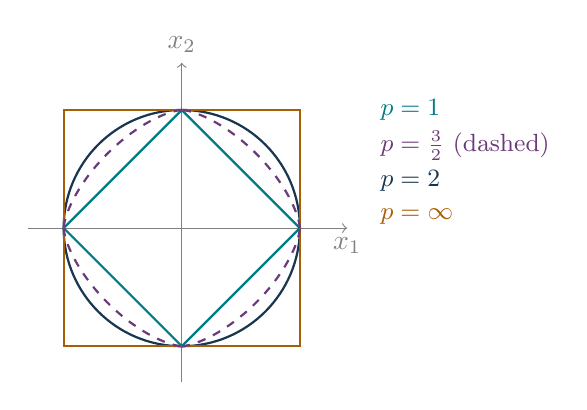
\begin{tikzpicture}[scale=1.5]
\draw[->,gray] (-1.3,0)--(1.4,0) node[below]{$x_1$};
\draw[->,gray] (0,-1.3)--(0,1.4) node[above]{$x_2$};
\draw[thick,teal] (1,0)--(0,1)--(-1,0)--(0,-1)--cycle;
\draw[thick,navy] (0,0) circle (1);
\draw[thick,amber] (-1,-1) rectangle (1,1);
\draw[thick,plum,dashed,domain=0:90,samples=60,smooth] plot ({cos(\x)^(4/3)},{sin(\x)^(4/3)});
\draw[thick,plum,dashed,domain=90:180,samples=60,smooth] plot ({-(-cos(\x))^(4/3)},{sin(\x)^(4/3)});
\draw[thick,plum,dashed,domain=180:270,samples=60,smooth] plot ({-(-cos(\x))^(4/3)},{-(-sin(\x))^(4/3)});
\draw[thick,plum,dashed,domain=270:360,samples=60,smooth] plot ({cos(\x)^(4/3)},{-(-sin(\x))^(4/3)});
\node[teal,anchor=west] at (1.6,1.0) {\small $p=1$};
\node[plum,anchor=west] at (1.6,0.7) {\small $p=\tfrac32$ (dashed)};
\node[navy,anchor=west] at (1.6,0.4) {\small $p=2$};
\node[amber,anchor=west] at (1.6,0.1) {\small $p=\infty$};
\end{tikzpicture}
\end{center}

\begin{exam}{Exercise 3.10 and 2025 Q3(c)}
(a) If $p\in B_r(a)\cap B_s(b)$, find $t>0$ with $B_t(p)\subset B_r(a)\cap B_s(b)$.
(b) If $x\ne y$ and $0<R\le d(x,y)/2$, show $B_R(x)\cap B_R(y)=\emptyset$.
\end{exam}
\begin{answer}
(a) Let $t=\min\{r-d(p,a),\,s-d(p,b)\}>0$. If $d(z,p)<t$ then
$d(z,a)\le d(z,p)+d(p,a)<r-d(p,a)+d(p,a)=r$, and similarly $d(z,b)<s$.\\
(b) If $z$ were in both, $d(x,y)\le d(x,z)+d(z,y)<2R\le d(x,y)$, a contradiction.
\end{answer}

\topic{Sequences in a metric space}
\begin{defn}{convergent, Cauchy, bounded}
$x_n\to a$ if $d(x_n,a)\to0$, i.e.\ $\forall\varepsilon>0\ \exists N\ \forall n\ge N$,
$d(x_n,a)<\varepsilon$. \textbf{Cauchy}: $\forall\varepsilon>0\ \exists N\ \forall n,m\ge N$,
$d(x_n,x_m)<\varepsilon$. \textbf{Bounded}: the set of terms is bounded.
\end{defn}
\begin{thm}{convergent $\Rightarrow$ Cauchy $\Rightarrow$ bounded (Exercise 3.11)}
In any metric space, every convergent sequence is Cauchy, and every Cauchy sequence is bounded.
\end{thm}
\begin{answer}
If $x_n\to a$, choose $N$ with $d(x_n,a)<\varepsilon/2$ for $n\ge N$; then
$d(x_n,x_m)\le d(x_n,a)+d(a,x_m)<\varepsilon$. If Cauchy, choose $N$ with $d(x_n,x_m)<1$ for
$n,m\ge N$. Then $d(x_n,x_N)\le M:=\max\{d(x_1,x_N),\dots,d(x_{N-1},x_N),1\}$ for all $n$, so
the terms lie in $B_{M}[x_N]$ and the sequence is bounded.
\end{answer}
Neither arrow reverses: $(1/n)$ in $\ro01$ is Cauchy but not convergent there; $(-1)^n$ is
bounded but not Cauchy.

\begin{exam}{convergence in a discrete space (2024 Q1 style)}
Show that in a discrete metric space a sequence converges iff it is eventually constant, and
that every Cauchy sequence converges.
\end{exam}
\begin{answer}
If $x_n\to p$, take $\varepsilon=\frac12$: there is $N$ with $d(x_n,p)<\frac12$ for $n\ge N$, and
the only distance below $\frac12$ is $0$, so $x_n=p$ for $n\ge N$. Conversely, if $x_n=p$ for
$n\ge N$ then $d(x_n,p)=0<\varepsilon$ for all $n\ge N$. The same $\varepsilon=\frac12$ argument
shows that a Cauchy sequence satisfies $x_n=x_N$ for all $n\ge N$, so it converges to $x_N$.
Hence discrete spaces are complete.
\end{answer}

\begin{example}{Exercise 3.12: convergence of metric values}
If $(x_n)$ is Cauchy, $|d(x_n,p)-d(x_m,p)|\le d(x_n,x_m)$ (reverse triangle inequality), so
$(d(x_n,p))$ is Cauchy in $\R$, hence convergent. If $x_n\to a$ then
$|d(x_n,p)-d(a,p)|\le d(x_n,a)\to0$.
\end{example}

\begin{tip}
\begin{itemize}
\item In (MS1) do \emph{both} directions; (MS1b) is where continuity or injectivity is used.
\item To disprove (MS3), give three explicit points. Example: $d(x,y)=(x-y)^2$ on $\R$ fails
  with $x=0,y=1,z=2$: $4>1+1$.
\item A metric subspace can look very different from the big space: the standard basis
  vectors in $\R^n$ form, with $d_2$, a copy of $\sqrt2\times$ the discrete metric.
\item $B_r(a)$ uses $<$; $B_r[a]$ uses $\le$. Don't mix them up.
\end{itemize}
\end{tip}

\section{Metric space topology: open, closed, continuity, density, equivalence (Section 4)}

\begin{plain}
``Topology'' is everything that can be described using \emph{open sets} alone: closed sets,
interior, closure, boundary, density, continuity, convergence. Two metrics that have the same
open sets (equivalent metrics) have the same topology, even if their distances are very different.
This is the most heavily examined Section. Every past paper had a full question on it.
\end{plain}

\topic{Open sets}
\begin{defn}{open set}
$U\subset E$ is \textbf{open} if $\forall p\in U\ \exists r>0$ with $B_r(p)\subset U$.
\emph{``Wherever you stand in $U$, there is a ball around you that stays inside $U$.''}
\end{defn}

\begin{exam}{open balls are open (2025 Q3(b) style)}
Prove that $B_R(a)$ is an open set.
\end{exam}
\begin{answer}
Let $p\in B_R(a)$ and set $r=R-d(p,a)>0$ (this is the ``spare radius''). If $x\in B_r(p)$, then
by (MS3) $d(x,a)\le d(x,p)+d(p,a)<r+d(p,a)=R$, so $x\in B_R(a)$. Hence $B_r(p)\subset B_R(a)$,
and $B_R(a)$ is open.
\end{answer}
\begin{center}
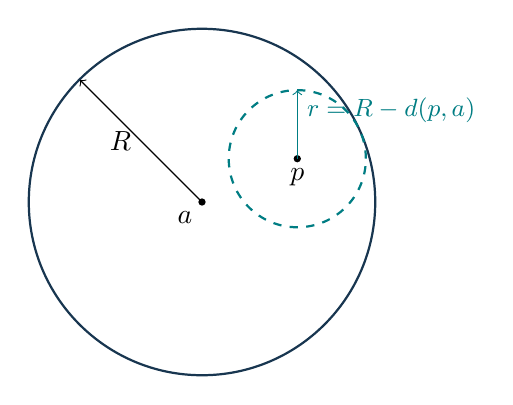
\begin{tikzpicture}[scale=1.1]
\draw[thick,navy] (0,0) circle (2); \fill (0,0) circle (1.2pt) node[below left]{$a$};
\fill (1.1,0.5) circle (1.2pt) node[below]{$p$};
\draw[thick,teal,dashed] (1.1,0.5) circle ({2-sqrt(1.1^2+0.5^2)});
\draw[->] (0,0)--(-1.41,1.41) node[midway,left]{$R$};
\draw[->,teal] (1.1,0.5)--++(0,{2-sqrt(1.1^2+0.5^2)}) node[right,pos=.7]{\small $r=R-d(p,a)$};
\end{tikzpicture}
\end{center}

\begin{thm}{the family of open sets $\mathcal O(E)$}
(a) $\emptyset$ and $E$ are open. (b) Any union of open sets is open.
(c) A \emph{finite} intersection of open sets is open (take $t=\min\{r_1,\dots,r_n\}$).
Every open set is a union of open balls: $U=\bigcup_{x\in U}B_{r(x)}(x)$.
\end{thm}
\textbf{Infinite intersections can fail}: $\bigcap_{n}\oi{-\frac1n}{\frac1n}=\{0\}$ is not open
in $\R$.

\begin{exam}{Exercises 4.1 and 4.2}
(a) What are the open sets in a discrete metric space? (b) If $V$ is open and $F$ finite, show
that $V\setminus F$ is open.
\end{exam}
\begin{answer}
(a) \emph{Every} subset $U$ is open: for $p\in U$, $B_1(p)=\{p\}\subset U$.\\
(b) Let $p\in V\setminus F$. Choose $r>0$ with $B_r(p)\subset V$. If $F=\emptyset$ we are done.
Otherwise $F=\{a_1,\dots,a_m\}$, and $\delta=\min_i d(p,a_i)>0$ because $p\notin F$ and the
minimum is over finitely many positive numbers. Let $t=\min\{r,\delta\}$. If $x\in B_t(p)$ then
$x\in V$, and $x\ne a_i$ because $d(x,p)<\delta\le d(a_i,p)$. So $B_t(p)\subset V\setminus F$.
(``Finite'' matters: $\R\setminus\{1/n:n\in\N\}$ is not open, since $0$ has no such ball.)
\end{answer}

\topic{Interior}
\begin{defn}{interior}
$p$ is an \textbf{interior point} of $A$ if $\exists r>0$ with $B_r(p)\subset A$.
$\inte A$ is the set of interior points. $\inte A=\bigcup\{U\subset A: U\text{ open}\}$, the
\emph{largest open subset} of $A$. So $\inte A$ is open, and $A$ is open $\iff A=\inte A$.
\end{defn}
Example: $\inte\Q=\emptyset$ in $\R$, since every interval $\oi{x-r}{x+r}$ contains an
irrational number.

\topic{Continuity}
\begin{defn}{continuity in metric spaces}
$f:E\to E'$ is \textbf{continuous at $p$} if $\forall\varepsilon>0\ \exists\delta>0$ with
$f(B_\delta(p))\subset B_\varepsilon(f(p))$. It is \textbf{sequentially continuous at $p$} if
$x_n\to p\Rightarrow f(x_n)\to f(p)$. These are equivalent. $f$ is continuous if it is continuous
at every point.
\end{defn}

\begin{thm}{global continuity via open sets (very frequently examined)}
$f:E\to E'$ is continuous $\iff$ $f^{-1}(V)$ is open in $E$ for every open $V\subset E'$
$\iff$ $f^{-1}(C)$ is closed in $E$ for every closed $C\subset E'$.
\end{thm}
\begin{answer}
\textbf{($\Rightarrow$)} Let $V\subset E'$ be open and $p\in f^{-1}(V)$. Then $f(p)\in V$, so
there is $\varepsilon>0$ with $B_\varepsilon(f(p))\subset V$. By continuity there is $\delta>0$
with $f(B_\delta(p))\subset B_\varepsilon(f(p))\subset V$. Hence $B_\delta(p)\subset f^{-1}(V)$,
so $f^{-1}(V)$ is open.\\
\textbf{($\Leftarrow$)} Let $p\in E$, $\varepsilon>0$. The ball $V=B_\varepsilon(f(p))$ is open,
so $f^{-1}(V)$ is open and contains $p$. Choose $\delta>0$ with $B_\delta(p)\subset f^{-1}(V)$.
Then $f(B_\delta(p))\subset V$, which is continuity at $p$.\\
\textbf{Closed version (Exercise 4.5).} $f^{-1}(E'\setminus C)=E\setminus f^{-1}(C)$, and a set
is closed iff its complement is open.
\end{answer}

\begin{tip}
Continuity is about \emph{preimages}. The \emph{image} of an open set under a continuous map
need not be open: the constant map $f\equiv0$ on $\R$ sends $\oi{-1}1$ to $\{0\}$, which is not
open. Likewise the image of a closed set need not be closed ($t\mapsto\frac1{1+t}$ sends
$\lo0\infty$ to $\ro01$).
\end{tip}

\textbf{Lipschitz $\Rightarrow$ continuous}: $f(B_r(p))\subset B_{Lr}(f(p))$ with $L=\Lip f$;
take $\delta=\varepsilon/L$. Compositions of continuous maps are continuous (Exercise 6.6:
$(g\circ f)^{-1}(W)=f^{-1}(g^{-1}(W))$).

\topic{Closed sets, closure}
\begin{thm}{point of closure: three equivalent conditions}
For $A\subset E$, $p\in E$, the following are equivalent:
(i) $\forall r>0$, $B_r(p)\cap A\ne\emptyset$; (ii) there is a sequence $(a_n)$ in $A$ with
$a_n\to p$; (iii) $\dist_A(p)=0$. Such a $p$ is a \textbf{point of closure} of $A$, and $\cl A$
is the set of all of them.
\end{thm}
\begin{defn}{closed set}
$A$ is \textbf{closed} if $\cl A=A$, i.e.\ \emph{whenever a sequence in $A$ converges in $E$,
its limit lies in $A$.}
\end{defn}

\begin{thm}{closed $\iff$ complement open}
$A$ is closed $\iff$ $E\setminus A$ is open.
\end{thm}
\begin{answer}
\textbf{Model proof (sequence version, 2025 Q3(e) style).}
($\Leftarrow$) Suppose $E\setminus A$ is open. Let $a_n\in A$ with $a_n\to p$. If $p\notin A$,
there is $r>0$ with $B_r(p)\subset E\setminus A$. Since $a_n\to p$, eventually $a_n\in B_r(p)$,
so $a_n\notin A$, a contradiction. So $p\in A$ and $A$ is closed.\\
($\Rightarrow$) Suppose $A$ is closed and $E\setminus A$ is not open. Then some
$p\in E\setminus A$ has $B_{1/n}(p)\cap A\ne\emptyset$ for every $n$. Pick $a_n$ in this
intersection. Then $a_n\to p$, $a_n\in A$, so $p\in A$ by closedness, a contradiction.
\end{answer}

\begin{thm}{the family of closed sets}
$\emptyset$, $E$ are closed; arbitrary \emph{intersections} and \emph{finite} unions of closed
sets are closed. $\cl A$ is closed and $\cl A=\bigcap\{F\supset A: F\text{ closed}\}$, the
\emph{smallest closed superset} of $A$. Also $\cl{\cl A}=\cl A$.
\end{thm}
\textbf{Infinite unions can fail}: $\bigcup_n[\frac1n,1]=\ro01$ is not closed.

\textbf{Complement identities}: $(\cl A)\cpl=\inte(A\cpl)$ and $(\inte A)\cpl=\cl{A\cpl}$.

\begin{thm}{closures of balls}
$\cl{B_r(a)}\subset B_r[a]$. Equality holds in normed spaces but can fail in general: in a
discrete space with $\ge2$ points, $\cl{B_1(a)}=\{a\}$ but $B_1[a]=E$.
\end{thm}
\begin{answer}
If $p\in\cl{B_r(a)}$, pick $x_n\in B_r(a)$ with $x_n\to p$. Then $d(x_n,a)\to d(p,a)$, and since
$d(x_n,a)<r$ for all $n$, order preservation gives $d(p,a)\le r$. \emph{(Only $\le$: strict
inequality is lost in the limit.)} Closed balls are closed by the same argument, and spheres are
closed too.
\end{answer}

\begin{exam}{closure of unions and intersections (2023 Q2(b) style)}
Prove $\cl{A\cup B}=\cl A\cup\cl B$. Give an example with $\cl{A\cap B}\subsetneq\cl A\cap\cl B$.
\end{exam}
\begin{answer}
$A\subset A\cup B$ gives $\cl A\subset\cl{A\cup B}$; similarly for $B$; so
$\cl A\cup\cl B\subset\cl{A\cup B}$. Conversely $\cl A\cup\cl B$ is closed (a finite union of
closed sets) and contains $A\cup B$, so it contains the smallest closed superset
$\cl{A\cup B}$. For the example, take $A=\oi01$, $B=\oi12$ in $\R$: $\cl{A\cap B}=\cl\emptyset
=\emptyset$, but $\cl A\cap\cl B=[0,1]\cap[1,2]=\{1\}$.
\end{answer}

\topic{Boundary}
\begin{defn}{boundary}
$\partial A=\cl A\setminus\inte A=\cl A\cap\cl{A\cpl}$. It is closed, and
$E=\inte A\ \sqcup\ \partial A\ \sqcup\ \inte(A\cpl)$ (disjoint union).
\end{defn}

\begin{steps}{finding interior, closure and boundary}
\begin{enumerate}
\item Draw the set. \textbf{Interior}: points with a whole ball inside $A$.
\item \textbf{Closure}: add all limits of sequences in $A$.
\item \textbf{Boundary}: closure minus interior. Check each claim with a ball or a sequence.
\end{enumerate}
\end{steps}

\begin{center}
\renewcommand{\arraystretch}{1.25}
\begin{tabular}{@{}lllll@{}}\toprule
Set $A$ (in $\R$ unless stated) & $\inte A$ & $\cl A$ & $\partial A$ & open/closed?\\\midrule
$\lo01$ & $\oi01$ & $[0,1]$ & $\{0,1\}$ & neither\\
$\lo01\cup\{2\}$ & $\oi01$ & $[0,1]\cup\{2\}$ & $\{0,1,2\}$ & neither\\
$\Q$ & $\emptyset$ & $\R$ & $\R$ & neither\\
$\{1/n:n\in\N\}$ & $\emptyset$ & $A\cup\{0\}$ & $A\cup\{0\}$ & neither\\
$\Z$ & $\emptyset$ & $\Z$ & $\Z$ & closed\\
$\R$, $\emptyset$ & itself & itself & $\emptyset$ & both\\
any $A$ in a discrete space & $A$ & $A$ & $\emptyset$ & both\\
$\{(x,y):x^2+y^2<1\}\subset\R^2$ & itself & closed disc & unit circle & open\\
\bottomrule\end{tabular}
\end{center}

\topic{Density and separability}
\begin{defn}{dense, separable}
$D$ is \textbf{dense} in $E$ if $\cl D=E$, i.e.\ every ball $B_R(p)$ meets $D$, i.e.\ every
$p\in E$ is a limit of a sequence in $D$. $E$ is \textbf{separable} if it has a
\emph{countable} dense subset.
\end{defn}
Examples: $\Q$ and $\R\setminus\Q$ are both dense in $\R$ (and disjoint). $\Q^N$ is dense in
$\ell^p(N)$, so $\R^N$ is separable. $C(I;\R)$ with $\dsup$ is separable (polynomials with
rational coefficients; or Exercise 4.11).

\begin{exam}{dense intersect open dense (2023 Q3(a) / 2024 Q2(d))}
Let $U$ be open and dense and $A$ dense in $E$. Prove that $U\cap A$ is dense. Show this can fail
if $U$ is not open.
\end{exam}
\begin{answer}
Let $p\in E$, $R>0$. We must show $B_R(p)\cap U\cap A\ne\emptyset$.
\begin{enumerate}
\item $U$ is dense, so there is $u\in B_R(p)\cap U$.
\item $B_R(p)\cap U$ is open (a finite intersection of open sets), so there is $r>0$ with
  $B_r(u)\subset B_R(p)\cap U$.
\item $A$ is dense, so there is $a\in B_r(u)\cap A$.
\item Then $a\in B_R(p)\cap U\cap A$.
\end{enumerate}
\textbf{Failure without openness}: $U=\Q$, $A=\R\setminus\Q$ are both dense in $\R$, but
$U\cap A=\emptyset$.
\end{answer}

\begin{exam}{a non-separable space}
Show that an uncountable set $S$ with the discrete metric is not separable.
\end{exam}
\begin{answer}
Let $D$ be dense. For each $s\in S$, the ball $B_1(s)=\{s\}$ must meet $D$, so $s\in D$. Thus
$D=S$, which is uncountable. So no countable dense subset exists.
\emph{(The same idea shows that $\ell^\infty(\N;\R)$, the bounded sequences with $\dsup$, is not
separable: the uncountably many $0$--$1$ sequences are pairwise at distance $1$, and the balls
$B_{1/2}$ around them are disjoint, so each must contain a different point of $D$.)}
\end{answer}

\begin{exam}{Exercise 4.11: a countable dense set in $C(I;\R)$ (2024 Q2(d)(v))}
Let $A_n$ be the continuous $g$ that are linear on each $[k/2^n,(k+1)/2^n]$ with
$g(j/2^n)\in\Q$, and $A=\bigcup_n A_n$. Show $A$ is countable and dense in $(C(I;\R),\dsup)$.
\end{exam}
\begin{answer}
\textbf{Countable.} $g\in A_n$ is determined by its values at the $2^n+1$ nodes, so
$g\mapsto(g(0),g(2^{-n}),\dots,g(1))$ is injective into $\Q^{2^n+1}$, which is countable. A
countable union of countable sets is countable.\\
\textbf{Dense.} Let $f\in C(I;\R)$, $\varepsilon>0$. By the Uniform Continuity Theorem choose
$n$ with $|f(s)-f(t)|<\varepsilon/3$ when $|s-t|\le2^{-n}$. Choose rationals $q_j$ with
$|q_j-f(j/2^n)|<\varepsilon/3$, and let $g\in A_n$ take these node values. For $t$ in a mesh
interval with nodes $s_0,s_1$, $g(t)$ is a convex combination of $q_0,q_1$, each within
$\varepsilon/3+\varepsilon/3$ of $f(t)$ (since $|q_i-f(t)|\le|q_i-f(s_i)|+|f(s_i)-f(t)|$).
So $|g(t)-f(t)|<2\varepsilon/3$ for all $t$, and $\dsup(f,g)\le2\varepsilon/3<\varepsilon$.
\end{answer}

\begin{thm}{open subsets of $\R$}
Every open $U\subset\R$ is a countable union of open intervals (those with rational endpoints
contained in $U$).
\end{thm}

\topic{Homeomorphisms}
\begin{defn}{homeomorphism}
$f:E\to E'$ is a \textbf{homeomorphism} if it is continuous, bijective, and $f^{-1}$ is
continuous. Equivalently: a continuous bijection that maps open sets to open sets.
\end{defn}
\textbf{Examples}: $\tan:\oi{-\pi/2}{\pi/2}\to\R$ (a bounded space homeomorphic to an unbounded
one). Bi-Lipschitz maps.\\
\textbf{Non-example}: $\id:(\R,d_{disc})\to(\R,|\cdot|)$ is a continuous bijection (every map
\emph{from} a discrete space is continuous, since every preimage is open), but its inverse is not
continuous: $\{0\}$ is open in the discrete space but not in $\R$.

\topic{Equivalent metrics}
\begin{defn}{topological and Lipschitz equivalence}
Metrics $d_1,d_2$ on $S$ are \textbf{topologically equivalent} if
$\id:(S,d_1)\to(S,d_2)$ is a homeomorphism; \textbf{Lipschitz equivalent} if it is
bi-Lipschitz, i.e.\ $\exists m,M>0$ with $m\,d_1\le d_2\le M\,d_1$.
Lipschitz equivalent $\Rightarrow$ topologically equivalent.
\end{defn}
\begin{thm}{tests for topological equivalence}
The following are equivalent: (i) $d_1,d_2$ topologically equivalent; (ii) they have the same
convergent sequences (with the same limits); (iii) they have the same closed sets; (iv) they have
the same open sets; (v) every $d_1$-ball about $p$ contains a $d_2$-ball about $p$, and vice versa.
\end{thm}
\begin{center}
\renewcommand{\arraystretch}{1.2}
\begin{tabular}{@{}lcc@{}}\toprule
Property & top.\ equiv.\ preserves? & Lipschitz equiv.\ preserves?\\\midrule
open and closed sets, convergence, density & yes & yes\\
sequential compactness & yes & yes\\
boundedness & \textbf{no} & yes\\
Cauchy sequences, completeness & \textbf{no} & yes\\\bottomrule
\end{tabular}
\end{center}

\begin{thm}{$\alpha\circ d$ is topologically equivalent to $d$}
If $\alpha$ is definite, increasing, subadditive and \emph{continuous at $0$}, then $\alpha\circ
d$ is a topologically equivalent metric. If moreover $\alpha$ is strictly increasing near $0$,
then $d$ and $\alpha\circ d$ have the same Cauchy sequences. Examples: $cs$, $\min\{s,1\}$,
$s/(1+s)$, $\tan^{-1}s$, $s^{1/p}$. \textbf{Corollary}: every metric is topologically equivalent
to a bounded metric with the same Cauchy sequences.
\end{thm}

\begin{exam}{truncated and arctangent metrics (2024 Q3(b)(c) style)}
(a) Show that $d'=\min\{d,1\}$ has the same convergent and the same Cauchy sequences as $d$.
(b) Show $d'$ and $d$ need not be Lipschitz equivalent.
(c) Show $d_{NS}(x,y)=|\tan^{-1}x-\tan^{-1}y|$ is topologically, but not Lipschitz, equivalent
to the usual metric on $\R$, and that $(\R,d_{NS})$ is not complete.
\end{exam}
\begin{answer}
(a) $d'\le d$, so $d$-convergent/Cauchy $\Rightarrow$ $d'$-convergent/Cauchy. Conversely, given
$0<\varepsilon<1$: once $d'(x_n,x_m)<\varepsilon<1$, the minimum must equal $d(x_n,x_m)$, so
$d(x_n,x_m)<\varepsilon$. The same holds for $d(x_n,a)$.\\
(b) On $\R$ with $d=|\cdot|$: if $d\le M\,d'$, then taking $x=0$, $y=n$ gives $n\le M$ for all
$n$, which is impossible. (In general: Lipschitz equivalence preserves boundedness, $d'$ is
bounded, and $d$ is not.)\\
(c) $\tan^{-1}:\R\to\oi{-\pi/2}{\pi/2}$ is a homeomorphism, so $x_n\to x$ in $|\cdot|$ $\iff$
$\tan^{-1}x_n\to\tan^{-1}x$ $\iff$ $x_n\to x$ in $d_{NS}$. Not Lipschitz equivalent: $d_{NS}<\pi$
is bounded, the usual metric is not. Not complete: $x_n=n$ is $d_{NS}$-Cauchy because
$\tan^{-1}n\to\pi/2$, so $d_{NS}(n,m)\le|\tan^{-1}n-\frac\pi2|+|\frac\pi2-\tan^{-1}m|\to0$. If
$n\to a$ in $d_{NS}$ then $\tan^{-1}n\to\tan^{-1}a$, so $\tan^{-1}a=\pi/2$, which is impossible.
\textbf{Moral: completeness is not a topological property.}
\end{answer}

\begin{exam}{Exercise 4.8: $d_{TGV}$ on $\R$}
$d_{TGV}(x,y)=|x|+|y|$ for $x\ne y$. Let $f=\id:(\R,|\cdot|)\to(\R,d_{TGV})$ and $g=f^{-1}$.
Show (a) $g$ is Lipschitz; (b) $f$ is continuous at $0$; (c) $f$ is not continuous at $a\ne0$.
\end{exam}
\begin{answer}
(a) $|x-y|\le|x|+|y|=d_{TGV}(x,y)$ for $x\ne y$, so $\Lip g\le1$.\\
(b) $d_{TGV}(x,0)=|x|$, so $|x-0|<\varepsilon\Rightarrow d_{TGV}(x,0)<\varepsilon$ ($\delta=\varepsilon$).\\
(c) Take $x_n=a+\frac1n\to a$ in $|\cdot|$. Then $d_{TGV}(x_n,a)=|x_n|+|a|\to2|a|\ne0$, so
$f(x_n)\not\to f(a)$. Hence $d_{TGV}$ is not topologically equivalent to the usual metric.
(Indeed $\{a\}=B^{TGV}_{|a|}(a)$ is $d_{TGV}$-open.)
\end{answer}

\textbf{All $\ell^p$ metrics on $\R^N$ are Lipschitz equivalent}, since
$\norm x_\infty\le\norm x_p\le N^{1/p}\norm x_\infty$. So in $\R^N$, open, closed, bounded,
convergent, Cauchy and compact do not depend on $p$, and convergence is coordinatewise.

\topic{Metric subspaces: ``open in $A$'' versus ``open in $E$''}
For $A\subset E$ with the restricted metric: $B^A_r(a)=A\cap B_r(a)$.
\begin{thm}{relatively open and closed sets}
For $X\subset A$: $X$ is open in $A$ $\iff$ $X=A\cap U$ for some $U$ open in $E$;
$X$ is closed in $A$ $\iff$ $X=A\cap F$ for some $F$ closed in $E$.
\end{thm}
\begin{answer}
\textbf{Proof of the open version (Exercise 4.10; 2022 Q2(d)).}
($\Leftarrow$) Let $v\in X=A\cap U$. Choose $r$ with $B_r(v)\subset U$. Then
$B^A_r(v)=A\cap B_r(v)\subset A\cap U=X$.\\
($\Rightarrow$) For each $v\in X$ choose $r_v>0$ with $B^A_{r_v}(v)\subset X$. Let
$U=\bigcup_{v\in X}B_{r_v}(v)$, which is open in $E$ as a union of balls. Each $v\in X$ is in
$A\cap U$. If $x\in A\cap U$ then $x\in A\cap B_{r_v}(v)=B^A_{r_v}(v)\subset X$ for some $v$.
So $X=A\cap U$.
\end{answer}

\begin{exam}{clopen in the subspace, neither in $E$ (2024 Q2(c)(ii))}
Give $A\subset E$ and $R\subset A$ such that $R$ is open and closed in $A$, but neither open nor
closed in $E$.
\end{exam}
\begin{answer}
$E=\R$, $A=R=\lo01$. The whole space is always open and closed in itself. In $\R$: not open,
since every ball about $0$ contains negative numbers; not closed, since $1-\frac1n\in R$
converges to $1\notin R$.
Another: in $A=\Z\subset\R$, $B^{\Z}_1(k)=\{k\}$, so every subset of $\Z$ is open and closed in
$\Z$.
\end{answer}

\begin{exam}{identity theorem (Exercise 6.7)}
Let $f,g:E\to E'$ be continuous. Show $H=\{x: f(x)=g(x)\}$ is closed, and that if $f=g$ on a
dense set then $f=g$.
\end{exam}
\begin{answer}
If $x_n\in H$, $x_n\to x$, then $f(x)=\lim f(x_n)=\lim g(x_n)=g(x)$ by sequential continuity and
uniqueness of limits, so $x\in H$. If $D\subset H$ is dense then $E=\cl D\subset\cl H=H$.
\end{answer}

\begin{tip}
\begin{itemize}
\item Always say \emph{where} a set is open or closed: ``open in $A$'' or ``open in $E$''.
\item To prove ``closed'' you may use sequences \emph{or} the complement. Pick the shorter route.
\item Many proofs need a radius $r$. Draw the picture and use the spare radius
  $R-d(p,a)$.
\item ``Dense'' means meets every ball. Prove it by fixing an arbitrary ball.
\item Completeness and boundedness are \emph{not} preserved by mere topological equivalence.
\end{itemize}
\end{tip}

\section{Complete metric spaces and the Contraction Mapping Theorem (Section 5)}

\begin{plain}
A space is \emph{complete} if it has no ``holes'': every sequence whose terms get closer and
closer together (Cauchy) actually converges to a point \emph{of the space}. $\R$ is complete;
$\Q$ is not (rational approximations to $\sqrt2$ have nowhere to converge). Completeness is the
hypothesis that makes the big existence theorems work: Banach's fixed point theorem, Cantor's
intersection theorem and Baire's theorem.
\end{plain}

\topic{Two basic facts about sequences}
\begin{thm}{uniqueness of limits; subsequences}
A sequence has at most one limit. Every subsequence of a convergent sequence converges to the
same limit.
\end{thm}
\begin{thm}{Cauchy with a convergent subsequence $\Rightarrow$ convergent}
If $(x_n)$ is Cauchy and $x_{n_k}\to a$, then $x_n\to a$.
\end{thm}
\begin{answer}
Let $\varepsilon>0$. Choose $N$ with $d(x_n,x_m)<\varepsilon$ for $n,m\ge N$, and $K$ with
$d(x_{n_K},a)<\varepsilon$ and $n_K\ge N$. Then for $n\ge N$:
$d(x_n,a)\le d(x_n,x_{n_K})+d(x_{n_K},a)<2\varepsilon$.
\end{answer}

\topic{Completeness: definition and examples}
\begin{defn}{complete}
$E$ is \textbf{complete} if every Cauchy sequence in $E$ converges (to a point of $E$).
\end{defn}
\begin{center}
\renewcommand{\arraystretch}{1.2}
\begin{tabular}{@{}ll@{}}\toprule
Complete & Not complete\\\midrule
$\R$, $\R^N$ with any $d_p$, $\C$ & $\Q$ \ (e.g.\ decimal truncations of $\sqrt2$)\\
closed subsets of complete spaces, e.g.\ $[0,1]$, $\Z$ & $\ro01$ \ ($x_n=1/n$)\\
discrete spaces & $(\R,d_{NS})$ \ ($x_n=n$)\\
$\ell^\infty(S;E)$ for complete $E$ & $(C([0,1];\R),d_1)$ (see below)\\
$C_b(E;E')$, $C(I;\R)$ with $\dsup$ & $\oi{-\pi/2}{\pi/2}$, although homeomorphic to $\R$\\
sequentially compact spaces & polynomials on $[0,1]$ with $\dsup$\\\bottomrule
\end{tabular}
\end{center}

\begin{steps}{showing a space is NOT complete}
Find a Cauchy sequence with no limit \emph{in the space}. Usually there is an ``obvious limit''
outside the space: show the sequence is Cauchy, then show that any limit in the space would
contradict uniqueness of limits in a bigger space.
\end{steps}

\begin{example}{$(C([0,1];\R),d_1)$ is not complete}
Let $f_n$ be $0$ on $[0,\frac12]$, $1$ on $[\frac12+\frac1n,1]$, and linear in between.
For $m\ge n$, $f_n$ and $f_m$ differ only on $[\frac12,\frac12+\frac1n]$, where both lie in
$[0,1]$, so $d_1(f_n,f_m)\le\frac1n$: the sequence is Cauchy. If $d_1(f_n,f)\to0$ with $f$
continuous, then on $[0,\frac12]$, $\int_0^{1/2}|f|\le d_1(f_n,f)\to0$, so $f=0$ there (by
Exercise 2.10). On $[\frac12+\delta,1]$ we have $f_n=1$ for $n>1/\delta$, so $f=1$ there for
every $\delta>0$. Then $f$ jumps at $\frac12$, which contradicts continuity.
\end{example}

\topic{Completeness and maps}
\begin{thm}{Lipschitz maps preserve Cauchy sequences (Exercise 5.1)}
If $\phi$ is Lipschitz, $d(\phi(x_n),\phi(x_m))\le L\,d(x_n,x_m)$, so $(\phi(x_n))$ is Cauchy when
$(x_n)$ is. Hence if $\phi:E\to E'$ is bi-Lipschitz, $E$ is complete $\iff E'$ is complete; and
Lipschitz equivalent metrics have the same complete spaces. The same proof works for
\emph{uniformly continuous} maps.
\end{thm}
\begin{answer}
\textbf{Bi-Lipschitz part.} Suppose $E'$ complete and $(x_n)$ Cauchy in $E$. Then $(\phi(x_n))$
is Cauchy in $E'$, so $\phi(x_n)\to y$. Then $x_n=\phi^{-1}(\phi(x_n))\to\phi^{-1}(y)$, since
$\phi^{-1}$ is Lipschitz and hence continuous. So $E$ is complete. The other direction is
symmetric.
\end{answer}

\begin{exam}{2022 Q3(b) style}
Let $f:E\to E'$ be a homeomorphism that is uniformly continuous, and let $E'$ be complete. Prove
that $E$ is complete. Why is ``homeomorphism'' alone not enough?
\end{exam}
\begin{answer}
Let $(x_n)$ be Cauchy in $E$ and $\varepsilon>0$. By uniform continuity there is $\delta>0$ with
$d(x,y)<\delta\Rightarrow d'(f(x),f(y))<\varepsilon$; choose $N$ with $d(x_n,x_m)<\delta$ for
$n,m\ge N$. Then $d'(f(x_n),f(x_m))<\varepsilon$, so $(f(x_n))$ is Cauchy in $E'$ and converges
to some $y$. As $f^{-1}$ is continuous, $x_n=f^{-1}(f(x_n))\to f^{-1}(y)\in E$. Hence $E$ is
complete.\\
\textbf{Not enough}: $\tan:\oi{-\pi/2}{\pi/2}\to\R$ is a homeomorphism onto the complete space
$\R$, but $\oi{-\pi/2}{\pi/2}$ is not complete. ($\tan$ is not uniformly continuous.)
\end{answer}

\topic{Complete $\iff$ closed (inside a complete space)}
\begin{thm}{closed subsets of complete spaces (2025 Q4(a))}
Let $A\subset E$ with the subspace metric. (i) If $A$ is complete then $A$ is closed in $E$.
(ii) If $E$ is complete and $A$ is closed in $E$, then $A$ is complete.
\end{thm}
\begin{answer}
(i) Let $a_n\in A$, $a_n\to p$ in $E$. Then $(a_n)$ is Cauchy (convergent sequences are
Cauchy), and the distances are the same in $A$, so $(a_n)$ is Cauchy in $A$. Since $A$ is
complete, $a_n\to a\in A$. By uniqueness of limits in $E$, $p=a\in A$. So $A$ is closed.\\
(ii) Let $(a_n)$ be Cauchy in $A$. It is Cauchy in $E$, which is complete, so $a_n\to p\in E$.
Since $A$ is closed, $p\in A$. Hence $(a_n)$ converges in $A$, and $A$ is complete.
\end{answer}
\textbf{Products}: a finite or countable product (with the metrics of Part 2) is complete iff
every factor is complete. Hence $\ell^p(N)$ is complete.

\topic{The paradigm theorem: $\ell^\infty(S;E)$ is complete}
\begin{thm}{completeness of $\ell^\infty(S;E)$}
If $E$ is complete then $(F_b(S;E),\dsup)$ is complete.
\end{thm}
\begin{answer}
\textbf{Model proof (2023 Q3(b), 2024 Q3(d); learn this one).}
\begin{enumerate}
\item \textbf{Pointwise Cauchy.} Let $(f_n)$ be $\dsup$-Cauchy. For each $s\in S$,
  $d(f_n(s),f_m(s))\le\dsup(f_n,f_m)$, so $(f_n(s))$ is Cauchy in $E$. As $E$ is complete,
  define $f(s):=\lim_n f_n(s)$.
\item \textbf{Uniform estimate (the crafty move).} Let $\varepsilon>0$ and choose $N$ with
  $\dsup(f_n,f_m)<\varepsilon$ for $n,m\ge N$. Then for every $s$ and $n,m\ge N$:
  $d(f_n(s),f_m(s))<\varepsilon$. Let $m\to\infty$ (the metric is continuous):
  \[d(f_n(s),f(s))\le\varepsilon\qquad\text{for all }s\in S,\ n\ge N.\tag{$*$}\]
\item \textbf{$f$ is bounded.} For $s,t\in S$:
  $d(f(s),f(t))\le d(f(s),f_N(s))+d(f_N(s),f_N(t))+d(f_N(t),f(t))\le2\varepsilon+\diam f_N(S)<\infty$.
  So $f\in F_b(S;E)$.
\item \textbf{Convergence.} By $(*)$, $\dsup(f_n,f)\le\varepsilon$ for $n\ge N$. So $f_n\to f$ in
  $\dsup$.
\end{enumerate}
\end{answer}

\begin{exam}{2024 Q3(d) style}
Show that $\ell^\infty(S;[0,1])$ is complete.
\end{exam}
\begin{answer}
$[0,1]$ is a closed subset of the complete space $\R$, hence complete. Apply the theorem.
(Every function into $[0,1]$ is automatically bounded.)
\end{answer}

\begin{thm}{$C_b(E;E')$ is complete (2025 Q4(b))}
If $E'$ is complete, the bounded continuous functions $C_b(E;E')$ with $\dsup$ form a complete
space. In particular $(C([0,1];\R),\dsup)$ is complete.
\end{thm}
\begin{answer}
By the closed-subset theorem it suffices to show $C_b(E;E')$ is \emph{closed} in the complete
space $\ell^\infty(E;E')$. Let $f_n\in C_b$, $\dsup(f_n,f)\to0$. Fix $x\in E$, $\varepsilon>0$.
Choose $N$ with $\dsup(f_N,f)<\varepsilon$, then $\delta>0$ with
$d(f_N(x),f_N(y))<\varepsilon$ whenever $d(x,y)<\delta$ (continuity of $f_N$). Then for such $y$:
\[d(f(x),f(y))\le d(f(x),f_N(x))+d(f_N(x),f_N(y))+d(f_N(y),f(y))<3\varepsilon.\]
So $f$ is continuous at $x$, and $f\in C_b$. (This is the ``$\varepsilon/3$ argument'': a uniform
limit of continuous functions is continuous.) For $C(I;\R)$: continuous functions on $[0,1]$ are
bounded, so $C(I;\R)=C_b(I;\R)$.
\end{answer}

\topic{Embedding, extension and completion (statements)}
\begin{thm}{embedding (proof not required from memory)}
Every metric space $E$ embeds isometrically into the complete normed space $\ell^\infty(E;\R)$.
If $E$ is bounded, use $x\mapsto d_x:=d(x,\cdot)$. In general, fix $\omega$ and use
$x\mapsto d_x-d_\omega$. Key inequality: $|d_x(p)-d_y(p)|\le d(x,y)$, with equality at $p=y$.
\end{thm}
\begin{thm}{unique Lipschitz extension}
If $E_0$ is dense in $E$, $E'$ is complete, and $f_0:E_0\to E'$ is Lipschitz, then $f_0$ has a
unique continuous extension $f:E\to E'$, given by $f(x)=\lim f_0(a_n)$ for any $a_n\to x$ with
$a_n\in E_0$. Moreover $\Lip f=\Lip f_0$, and $f$ is an isometry if $f_0$ is. (Same with
``uniformly continuous'', Exercise 5.9.)
\end{thm}
\textbf{Idea of proof}: $(a_n)$ is Cauchy $\Rightarrow$ $(f_0(a_n))$ is Cauchy $\Rightarrow$ it
converges (completeness). Two sequences tending to $x$ give the same limit, so $f$ is
well defined. Lipschitz bounds pass to the limit. Uniqueness comes from the identity theorem.

\begin{defn}{completion}
A completion of $E$ is a complete space $\tilde E$ with an isometry $\iota:E\to\tilde E$ whose
range is dense. Completions exist and are unique up to a unique isometry (proof
\textbf{non-examinable}). Example: the completion of $\Q$ is $\R$; of $(C(I;\R),d_1)$ it is
$L^1(I)$ (optional).
\end{defn}

\topic{Banach's Contraction Mapping Theorem}
\begin{thm}{Banach's CMT}
Let $E$ be a \textbf{nonempty complete} metric space and $\phi:E\to E$ a \textbf{strict
contraction} ($d(\phi(x),\phi(y))\le L\,d(x,y)$ with $L<1$). Then $\phi$ has a \textbf{unique}
fixed point $a$, and for every $x\in E$, $\phi^{\circ n}(x)\to a$.
\end{thm}
\begin{answer}
\textbf{Proof (learn it; it is examinable and often asked).}
\begin{enumerate}
\item \textbf{Uniqueness.} If $\phi(a)=a$, $\phi(b)=b$, $a\ne b$, then
  $d(a,b)=d(\phi(a),\phi(b))\le L\,d(a,b)<d(a,b)$, a contradiction.
\item \textbf{The iterates are Cauchy.} Let $x_0=x$, $x_k=\phi(x_{k-1})$. By induction
  $d(x_k,x_{k+1})\le L^k d(x_0,x_1)$. For $n,p\ge1$, by the triangle inequality,
  \[d(x_n,x_{n+p})\le\sum_{k=n}^{n+p-1}L^kd(x_0,x_1)\le\frac{L^n}{1-L}\,d(x_0,x_1)\to0.\]
\item \textbf{Limit.} $E$ is complete, so $x_n\to a$. $\phi$ is Lipschitz, hence continuous, so
  $\phi(a)=\lim\phi(x_n)=\lim x_{n+1}=a$.
\end{enumerate}
\textbf{Error estimate} (useful in numerical questions): letting $p\to\infty$,
$d(x_n,a)\le\frac{L^n}{1-L}d(x_0,x_1)$.
\end{answer}

\begin{center}
\renewcommand{\arraystretch}{1.2}
\begin{tabular}{@{}lll@{}}\toprule
Hypothesis dropped & Counterexample & Why it fails\\\midrule
completeness & $\phi(x)=x/2$ on $\ro01$ & fixed point $0$ is missing\\
$L<1$ (only $L=1$) & $\phi(x)=x+1$ on $\R$ & no fixed point\\
$L<1$ (only $d(\phi x,\phi y)<d(x,y)$) & $\phi(x)=x+\frac1x$ on $\lo1\infty$ & $x=x+\frac1x$ impossible\\
$\phi(E)\subset E$ & $\phi(x)=\frac x2+1$ on $[0,1]$ & $\phi(1)=\frac32\notin[0,1]$\\\bottomrule
\end{tabular}
\end{center}
\emph{Check of the third row}: for $x\ne y\ge1$,
$|\phi(x)-\phi(y)|=|x-y|\,\big|1-\frac1{xy}\big|<|x-y|$, and $[1,\infty[$ is closed in $\R$, hence
complete.

\begin{exam}{solving $\cos x=x$}
Show that $\cos x=x$ has exactly one solution in $[0,1]$, and that the iteration
$x_{n+1}=\cos x_n$ converges to it from any $x_0\in[0,1]$.
\end{exam}
\begin{answer}
$E=[0,1]$ is closed in $\R$, so complete. $\phi=\cos$ maps $[0,1]$ into $[\cos1,1]\subset[0,1]$.
By the mean value theorem, $|\cos x-\cos y|=|\sin\xi||x-y|\le\sin(1)|x-y|$ for some $\xi$ between
$x,y$, and $L=\sin1\approx0.84<1$. By Banach's CMT there is a unique fixed point in $[0,1]$, and
the iterates converge to it. (Any solution of $\cos x=x$ in $\R$ lies in $[-1,1]$, and on
$[-1,0[$ we have $\cos x>0>x$; so it is in fact the unique real solution.)
\end{answer}

\begin{exam}{an integral equation}
Show there is a unique $y\in C([0,1];\R)$ with $y(t)=1+\frac12\int_0^t y(s)\,ds$ for all $t$.
Identify $y$.
\end{exam}
\begin{answer}
Let $E=(C([0,1];\R),\dsup)$, which is complete. Define $\phi(f)(t)=1+\frac12\int_0^tf$. The map
$t\mapsto\int_0^tf$ is continuous (it is Lipschitz with constant $\norm f_{\sup}$), so
$\phi(f)\in E$. For $f,g\in E$ and $t\in[0,1]$:
\[|\phi(f)(t)-\phi(g)(t)|\le\tfrac12\int_0^t|f-g|\le\tfrac12\,t\,\dsup(f,g)\le\tfrac12\dsup(f,g).\]
So $\dsup(\phi f,\phi g)\le\frac12\dsup(f,g)$, a strict contraction. By Banach there is a unique
fixed point $y$. Since $y'=\frac12y$, $y(0)=1$ (FTC), we get $y(t)=e^{t/2}$; check:
$1+\frac12\int_0^te^{s/2}ds=1+(e^{t/2}-1)=e^{t/2}$.\\
\textbf{General version in the notes}: for $y(t)=\alpha(t)+\int_a^t\beta(y(s),s)ds$ with $\beta$
Lipschitz in its first variable (constant $M$), one gets
$\dsup(\phi^{\circ n}f,\phi^{\circ n}g)\le\frac{(M(b-a))^n}{n!}\dsup(f,g)$, and the extended CMT
(Exercise 5.4: $\sum\alpha_n<\infty$) applies on any interval, however long.
\end{answer}

\begin{exam}{a power of $T$ is a contraction (2022 Q3(c)(ii))}
Let $E$ be nonempty and complete, $T:E\to E$, and suppose $S=T^{\circ K}$ is a strict contraction.
Show $T$ has a unique fixed point $p$ and $T^{\circ n}x\to p$ for all $x$.
\end{exam}
\begin{answer}
By Banach, $S$ has a unique fixed point $p$. Since $S\circ T=T\circ S$:
$S(Tp)=T(Sp)=Tp$, so $Tp$ is a fixed point of $S$, and by uniqueness $Tp=p$. Any fixed point of
$T$ is a fixed point of $S$, hence equals $p$. For $r\in\{0,\dots,K-1\}$,
$T^{\circ(mK+r)}x=S^{\circ m}(T^{\circ r}x)\to p$ as $m\to\infty$. Finitely many subsequences
covering all $n$ tend to $p$, so $T^{\circ n}x\to p$.
\end{answer}

\topic{Cantor's Intersection Theorem}
\begin{thm}{Cantor's Intersection Theorem}
Let $E$ be complete and $F_1\supset F_2\supset\cdots$ \textbf{nonempty, closed} sets with
$\diam F_n\to0$. Then $\bigcap_nF_n$ is a single point.
\end{thm}
\begin{answer}
At most one point: $\diam\bigcap F_n\le\diam F_n\to0$. At least one: choose $x_n\in F_n$. For
$p\ge0$, $x_{n+p}\in F_n$, so $d(x_n,x_{n+p})\le\diam F_n\to0$: Cauchy. By completeness
$x_n\to a$. For fixed $n$, $(x_{n+p})_p$ lies in the closed set $F_n$, so $a\in F_n$. Hence
$a\in\bigcap F_n$.
\end{answer}
\textbf{Every hypothesis is needed (Exercise 5.6)}: drop closed: $F_n=\oi0{1/n}$ in $\R$ (empty
intersection). Drop $\diam\to0$: $F_n=\lo n\infty$ (closed, nested, empty intersection). Drop
completeness: $F_n=\Q\cap[\sqrt2-\frac1n,\sqrt2+\frac1n]$ in $\Q$.

\topic{Baire Category Theorem (proof non-examinable)}
\begin{thm}{Baire}
In a complete metric space, a countable intersection of open dense sets is dense. Equivalently,
a countable union of closed nowhere dense sets ($\inte\cl A=\emptyset$) has dense complement; in
particular a complete space is not such a union.
\end{thm}
Consequences: $\R$ is uncountable (it is not a countable union of points); $\R^2$ is not a
countable union of lines; ``most'' continuous functions are nowhere differentiable.

\begin{exam}{Exercise 5.7: what ``not Cauchy'' means}
Show $(x_n)$ is not Cauchy iff it has a subsequence with $\inf_kd(x_{n_k},x_{n_{k+1}})>0$.
\end{exam}
\begin{answer}
First, Cauchy $\iff\forall\varepsilon\ \exists N\ \forall n\ge N$, $d(x_N,x_n)<\varepsilon$
(use $\varepsilon/2$ and the triangle inequality for ``$\Leftarrow$''). So not Cauchy means:
$\exists\varepsilon_0>0\ \forall N\ \exists n\ge N$ with $d(x_N,x_n)\ge\varepsilon_0$. Set $n_1=1$
and choose $n_{k+1}$ with $d(x_{n_k},x_{n_{k+1}})\ge\varepsilon_0$, which forces
$n_{k+1}>n_k$. The infimum is $\ge\varepsilon_0$. Conversely, if the infimum is $\eta>0$ and
the sequence were Cauchy, choose $N$ for $\eta/2$ and $k$ with $n_k\ge N$: then
$\eta\le d(x_{n_k},x_{n_{k+1}})<\eta/2$, a contradiction.
\end{answer}

\begin{tip}
\begin{itemize}
\item In completeness proofs, the candidate limit comes from completeness of the
  \emph{target} space, applied pointwise. Then you must prove (a) it is in the space and (b)
  convergence happens in \emph{the given metric}, not just pointwise.
\item ``Let $m\to\infty$ in $d(f_n(s),f_m(s))<\varepsilon$'' gives $\le\varepsilon$, not $<$.
\item Banach: check all four conditions: nonempty, complete, maps \emph{into itself},
  constant $L<1$. A Lipschitz constant of exactly $1$ is not enough.
\item Completeness is a \emph{metric} property, not topological: $\R$ and
  $\oi{-\pi/2}{\pi/2}$ are homeomorphic, but only one is complete.
\end{itemize}
\end{tip}

\section{Sequential compactness, Heine--Borel and the Cantor set (Section 6)}

\begin{plain}
A set is \emph{sequentially compact} if no sequence in it can ``escape'': every sequence has a
subsequence that settles down to a point \emph{of the set}. Closed bounded intervals are the
model (Bolzano--Weierstrass). Compactness is what makes continuous functions attain their max and
min, and makes continuous bijections into homeomorphisms. In $\R^N$ it is the same as ``closed
and bounded'' (Heine--Borel), but in general spaces it is strictly stronger.
\end{plain}

\topic{Definition and first properties}
\begin{defn}{sequentially compact}
$K\subset E$ is \textbf{sequentially compact} if every sequence in $K$ has a subsequence that
converges to a limit \emph{in $K$}.
\end{defn}

\begin{thm}{sequentially compact $\Rightarrow$ closed and bounded}
If $K\subset E$ is sequentially compact, then $K$ is closed in $E$ and bounded.
\end{thm}
\begin{answer}
\textbf{Closed.} Let $x_n\in K$, $x_n\to a$ in $E$. A subsequence converges to some $b\in K$;
but every subsequence also converges to $a$, so $a=b\in K$.\\
\textbf{Bounded.} If not, build $x_1\in K$ and then $x_{k+1}\in K$ with $d(x_{k+1},x_i)\ge1$ for
all $i\le k$. (Possible: if every point of $K$ were within $1$ of $\{x_1,\dots,x_k\}$, $K$ would
be bounded.) Then $d(x_n,x_m)\ge1$ for $n\ne m$, so no subsequence is Cauchy, and none converges.
\end{answer}

\begin{thm}{more basic facts}
\begin{enumerate}
\item \textbf{Intrinsic}: $K$ is sequentially compact in $E$ iff it is sequentially compact as a
  space in its own right. (Unlike ``open'' or ``closed''.)
\item \textbf{Compact $\Rightarrow$ complete}: a Cauchy sequence with a convergent subsequence
  converges.
\item \textbf{Closed subsets}: if $E$ is sequentially compact, $F\subset E$ is sequentially
  compact $\iff$ $F$ is closed.
\item Finite sets, finite unions and arbitrary intersections of sequentially compact sets
  are sequentially compact (Exercise 6.1).
\end{enumerate}
\end{thm}

\begin{exam}{2022 Q4(a): closed subsets of compact spaces}
Let $K$ be sequentially compact and $A\subset K$. Prove $A$ is sequentially compact iff $A$ is
closed in $K$.
\end{exam}
\begin{answer}
($\Rightarrow$) As above: compact sets are closed.\\
($\Leftarrow$) Let $(a_n)$ be a sequence in $A$. It lies in $K$, so a subsequence
$a_{n_j}\to x\in K$. The subsequence lies in $A$ and $A$ is closed, so $x\in A$. Hence $A$ is
sequentially compact.
\end{answer}

\begin{exam}{Exercise 6.1}
Show (a) $A\cup B$, (b) $A\cap B$ are sequentially compact if $A,B$ are, and (c) finite sets are
sequentially compact.
\end{exam}
\begin{answer}
(a) A sequence in $A\cup B$ has infinitely many terms in $A$ or in $B$, say $A$. Those terms form
a subsequence in $A$, which has a further subsequence converging in $A\subset A\cup B$.\\
(b) $A\cap B$ is closed (as $B$ is closed) and is a subset of the compact set $A$; it is also
closed in $A$. Apply 2022 Q4(a).\\
(c) A sequence in a finite set takes some value infinitely often; that constant subsequence
converges.
\end{answer}

\topic{Continuous images: the most useful theorem}
\begin{thm}{continuous image of compact is compact}
If $f:E\to E'$ is continuous and $K\subset E$ is sequentially compact, then $f(K)$ is
sequentially compact (hence closed and bounded).
\end{thm}
\begin{answer}
Let $(y_n)$ be in $f(K)$; write $y_n=f(x_n)$ with $x_n\in K$. Then $x_{n_k}\to a\in K$, so by
sequential continuity $y_{n_k}=f(x_{n_k})\to f(a)\in f(K)$.
\end{answer}

\begin{thm}{consequences}
\begin{enumerate}
\item \textbf{Extreme value theorem} (Exercise 6.3): a continuous $f:K\to\R$ on a nonempty
  sequentially compact $K$ attains its max and min.
\item \textbf{Realisation} (6.2): there are $a,b\in K$ with $d(a,b)=\diam K$; for $p\in E$
  there is $c\in K$ with $d(c,p)=\dist_K(p)$.
\item \textbf{Continuous bijection from a compact space is a homeomorphism.}
\item \textbf{Compactness is topological}: topologically equivalent metrics have the same
  sequentially compact sets.
\end{enumerate}
\end{thm}
\begin{answer}
\textbf{1.} $f(K)\subset\R$ is compact, so closed and bounded. Let $u=\sup f(K)$. There is a
sequence in $f(K)$ tending to $u$ (approximation of suprema), and $f(K)$ is closed, so
$u\in f(K)$, i.e.\ $u=f(q)$. Similarly for the inf.\\
\textbf{2.} $\dist_K$ is continuous ($1$-Lipschitz), so it attains its min on $K$ by 1. For the
diameter, pick $(a_n,b_n)$ with $d(a_n,b_n)\to\diam K$; $K\times K$ is compact (product theorem),
so a subsequence converges to $(a,b)$, and by continuity of $d$, $d(a,b)=\diam K$.\\
\textbf{3.} Let $g=f^{-1}$. For $F\subset E$ closed: $F$ is compact (closed in compact), so
$g^{-1}(F)=f(F)$ is compact, hence closed. So $g$ is continuous (preimages of closed sets are
closed).
\end{answer}

\begin{exam}{what continuous maps preserve (2023 Q4(a) style)}
Give examples showing that a continuous image of a bounded set need not be bounded, and of a
closed set need not be closed. Then show that if $A\subset\R^2$ is closed and bounded and
$f:A\to E$ is continuous, $f(A)$ is closed and bounded.
\end{exam}
\begin{answer}
\textbf{Bounded $\not\to$ bounded}: $f(t)=1/t$ on the bounded set $\ro01$ has image
$\lo1\infty$; or $\tan$ on $\oi{-\pi/2}{\pi/2}$ has image $\R$.
\textbf{Closed $\not\to$ closed}: $f(t)=\frac1{1+t}$ on the closed set $\lo0\infty$ has image
$\ro01$, which is not closed.\\
\textbf{Closed and bounded}: by Heine--Borel $A$ is sequentially compact; so $f(A)$ is
sequentially compact; so $f(A)$ is closed and bounded.
\end{answer}

\begin{example}{optimisation using compactness}
$K=\{(x,y):x^2+y^2\le4,\ y\ge0\}$ is closed (an intersection of preimages of closed sets under
continuous maps) and bounded, so it is compact by Heine--Borel. Then $f(x,y)=x+y$ attains a max
and a min on $K$. On the arc $(2\cos\theta,2\sin\theta)$, $0\le\theta\le\pi$:
$f=2\sqrt2\sin(\theta+\frac\pi4)$, max $2\sqrt2$ at $(\sqrt2,\sqrt2)$. On the segment $y=0$:
$f=x\ge-2$. Since $f$ is linear, its extremes over $K$ occur on the boundary. So $\max=2\sqrt2$,
$\min=-2$ at $(-2,0)$.
\end{example}

\topic{Products and Heine--Borel}
\begin{thm}{Tychonoff (countable, metric version)}
A countable product of sequentially compact spaces, with the metric
$\sum_k d'_k(x_k,y_k)$ ($d'_k$ equivalent to $d_k$, $\sum\diam_{d'_k}<\infty$), is sequentially
compact. ``Baby Tychonoff'': the same for finite products with the sum metric.
\end{thm}
\textbf{Proof idea (diagonal argument).} Take a subsequence converging in coordinate $1$; from it
a further subsequence converging in coordinate $2$; and so on. The diagonal sequence (the $k$-th
term of the $k$-th subsequence) is eventually a subsequence of each of these, so it converges in
every coordinate. Convergence in every coordinate means convergence in the product.

\begin{thm}{Heine--Borel}
For $A\subset\R^N$ (with any $\ell^p$ metric): $A$ is sequentially compact $\iff$ $A$ is closed
and bounded.
\end{thm}
\begin{answer}
($\Rightarrow$) always true. ($\Leftarrow$) $A$ bounded $\Rightarrow$ $A\subset[-L,L]^N$ for some
$L$ (Exercise 6.4: if $\diam_\infty A=D$, fix $a\in A$; then $|x_i|\le\norm a_\infty+D$). By
Bolzano--Weierstrass $[-L,L]$ is sequentially compact, so $[-L,L]^N$ is too (Baby Tychonoff). $A$
is a closed subset of this compact set, so it is sequentially compact. All $\ell^p$ metrics are
Lipschitz equivalent, so nothing depends on $p$.
\end{answer}

\begin{tip}
\textbf{Heine--Borel is false in general metric spaces.} Closed and bounded does not imply
compact:
\begin{itemize}
\item $\N$ with the discrete metric: closed, bounded ($\diam=1$), but $(n)$ has no convergent
  subsequence (convergent sequences are eventually constant).
\item The closed unit ball of $(C([0,1];\R),\dsup)$: $f_n(x)=x^n$ has $\dsup(f_n,0)=1$. If
  $f_{n_k}\to g$ uniformly, then $g$ is continuous and equals the pointwise limit, which is
  $0$ on $\lo01$ and $1$ at $1$. That limit is not continuous, so no subsequence converges.
\item The unit ball of $\ell^\infty(\N;\R)$: $e_n$ (1 in place $n$, else 0) has
  $\dsup(e_n,e_m)=1$ for $n\ne m$.
\end{itemize}
\end{tip}

\begin{exam}{compact unit ball (2024 Q4(b) style)}
Let $X$ be a normed space whose closed unit ball $B_1[0]$ is sequentially compact. Prove that
every closed bounded subset of $X$ is sequentially compact.
\end{exam}
\begin{answer}
Let $A$ be closed and bounded, so $A\subset B_R[0]$ for some $R>0$. The map $h(x)=Rx$ is
continuous ($\norm{h(x)-h(y)}=R\norm{x-y}$) and maps $B_1[0]$ onto $B_R[0]$ (for $\norm y\le R$,
$y=h(y/R)$). So $B_R[0]$ is sequentially compact as a continuous image. $A$ is closed in $X$,
hence closed in $B_R[0]$, so $A$ is sequentially compact.
\end{answer}

\begin{exam}{isometries of a compact space (2022 Q4(c) style)}
Let $E$ be sequentially compact and $f:E\to E$ an isometry. Prove $f$ is surjective, hence a
homeomorphism.
\end{exam}
\begin{answer}
Let $p\in E$. The sequence $(f^{\circ n}(p))_{n\ge1}$ has a convergent subsequence
$(f^{\circ n_j}(p))$, which is Cauchy, so $d(f^{\circ n_{j+1}}(p),f^{\circ n_j}(p))\to0$. As
$f^{\circ n_j}$ is an isometry, this distance equals $d(f^{\circ m_j}(p),p)$ with
$m_j=n_{j+1}-n_j\ge1$. Hence $f^{\circ m_j}(p)\to p$. Each $f^{\circ m_j}(p)$ lies in $f(E)$,
which is compact (a continuous image), hence closed. So $p\in f(E)$. Thus $f$ is surjective; it
is injective (isometry), and $f^{-1}$ is an isometry, so continuous. So $f$ is a homeomorphism.
\end{answer}

\begin{exam}{Exercise 6.5}
If $x_n\to a$, show $C=\{a\}\cup\{x_n:n\in\N\}$ is closed. (In fact it is compact.)
\end{exam}
\begin{answer}
We show $E\setminus C$ is open. Let $y\notin C$; then $r:=d(y,a)/2>0$. Choose $N$ with
$d(x_n,a)<r$ for $n\ge N$; then $d(x_n,y)\ge d(y,a)-d(x_n,a)>r$ for $n\ge N$. Let
$t=\min\{r,d(y,x_1),\dots,d(y,x_{N-1})\}>0$ (each is positive since $y\notin C$). Then $B_t(y)$
misses $a$ (as $t<2r$) and every $x_n$, so $B_t(y)\subset E\setminus C$.
\end{answer}

\topic{The Cantor middle-thirds set $Z$}
Start with $Z_0=[0,1]$ and remove open middle thirds:
$Z_n=\alpha(Z_{n-1})\cup\beta(Z_{n-1})$ with $\alpha(x)=x/3$, $\beta(x)=x/3+2/3$.
$Z_n$ is $2^n$ disjoint closed intervals of length $3^{-n}$. Set $Z=\bigcap_nZ_n$.

\begin{center}
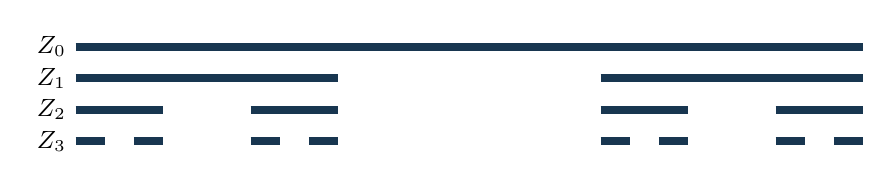
\begin{tikzpicture}[xscale=10,yscale=0.4]
\foreach \lev in {0,1,2,3}{
  \pgfmathsetmacro{\y}{-\lev}
  \node[left] at (0,\y) {\small $Z_{\lev}$};
}
\draw[line width=3pt,navy] (0,0)--(1,0);
\draw[line width=3pt,navy] (0,-1)--(1/3,-1) (2/3,-1)--(1,-1);
\draw[line width=3pt,navy] (0,-2)--(1/9,-2) (2/9,-2)--(1/3,-2) (2/3,-2)--(7/9,-2) (8/9,-2)--(1,-2);
\foreach \a in {0,2/9,2/3,8/9}{
  \draw[line width=3pt,navy] (\a,-3)--(\a+1/27,-3) (\a+2/27,-3)--(\a+1/9,-3);
}
\end{tikzpicture}
\end{center}

\begin{thm}{properties of $Z$}
\begin{enumerate}
\item $Z=\{2\sum_{n\ge1}c_n3^{-n}:c_n\in\{0,1\}\}$: the numbers in $[0,1]$ with a ternary
  expansion using only digits $0$ and $2$.
\item $Z$ is closed (an intersection of finite unions of closed intervals) and bounded, so
  sequentially compact.
\item $Z$ is homeomorphic to the Cantor space $\mathcal C=\{0,1\}^\N$ with
  $d(x,y)=\sum2^{-n}|y_n-x_n|$, via $\phi(x)=2\sum x_n3^{-n}$.
\item $Z$ is uncountable (it is in bijection with $\{0,1\}^\N$).
\item $Z$ is nowhere dense ($\inte Z=\emptyset$, as $Z$ contains no interval of length
  $>3^{-n}$ for any $n$).
\item $Z$ has length $0$: $Z\subset Z_n$, which has total length $(2/3)^n\to0$.
\end{enumerate}
So $Z$ is large as a set (uncountable) but small topologically and in length.
\end{thm}
\begin{answer}
\textbf{Why $\phi$ is a homeomorphism.} \emph{Lipschitz}: $|\phi(y)-\phi(x)|\le2\sum
\frac{|y_n-x_n|}{3^n}\le2\sum\frac{|y_n-x_n|}{2^n}=2d(x,y)$. \emph{Surjective}: by property 1.
\emph{Injective}: if $N$ is the first index with $x_N=0$, $y_N=1$, then the tail of $\phi(x)$
after place $N-1$ is at most $2\sum_{n>N}3^{-n}=3^{-N}<2\cdot3^{-N}\le$ the tail of $\phi(y)$,
so $\phi(x)<\phi(y)$. $\mathcal C$ is sequentially compact (a countable product of the finite
spaces $\{0,1\}$), so the continuous bijection $\phi$ is a homeomorphism.
\end{answer}

\begin{example}{Exercise 6.8: Cauchy via tails}
Let $X_n=\{x_k:k\ge n\}$. Then $(x_n)$ is Cauchy $\iff\diam X_n\to0$: ``$d(x_k,x_m)<\varepsilon$
for $k,m\ge N$'' says exactly ``$\diam X_N\le\varepsilon$'', and $\diam X_n$ decreases in $n$.
\end{example}

\begin{example}{Exercise 6.9: pseudo-metric to metric}
If $\rho$ satisfies all metric axioms except definiteness, $x\sim y\iff\rho(x,y)=0$ is an
equivalence relation (transitivity: $\rho(x,z)\le\rho(x,y)+\rho(y,z)=0$), and
$d([x],[y])=\rho(x,y)$ is well defined: if $x\sim x'$, $y\sim y'$ then
$|\rho(x,y)-\rho(x',y')|\le\rho(x,x')+\rho(y,y')=0$ by the four-point estimate. It is then a
metric. For $\rho(f,g)=\int_a^b|g-f|$ on Riemann integrable functions, $f=\mathbf 1_{\{a\}}$
and $g=0$ have $\rho=0$ but $f\ne g$.
\end{example}

\begin{tip}
\begin{itemize}
\item The limit of the subsequence must be \emph{in $K$}. ``Every sequence has a convergent
  subsequence'' with the limit outside $K$ is not enough: $\ro01$ fails this.
\item Use Heine--Borel only in $\R^N$. In other spaces, prove compactness directly, or via
  continuous images, closed subsets and products.
\item A continuous bijection is a homeomorphism automatically \emph{only} when the domain is
  compact.
\end{itemize}
\end{tip}

\section{Exam question bank: easy to hard, with model answers}

\begin{plain}
These questions are in the style of the 2022--2025 papers. They are graded
\textbf{Easy} (definitions and one-step checks), \textbf{Medium} (standard proofs using one
template) and \textbf{Hard} (several ideas combined, or unfamiliar settings). Cover the answer,
write your own, then compare. Questions already worked earlier in the guide are not repeated,
but are listed at the end of this Part.
\end{plain}

\topic{Easy}

\begin{exam}{E1: which formulas are metrics on $\R$?}
(a) $|x^2-y^2|$ \quad (b) $(x-y)^2$ \quad (c) $\sqrt{|x-y|}$ \quad (d) $|x-2y|$ \quad
(e) $\min\{|x-y|,1\}$ \quad (f) $|x^3-y^3|$
\end{exam}
\begin{answer}
(a) \textbf{No}: (MS1b) fails, $d(1,-1)=0$ but $1\ne-1$.
(b) \textbf{No}: (MS3) fails with $0,1,2$: $d(0,2)=4>1+1$.
(c) \textbf{Yes}: $\alpha(t)=\sqrt t$ is definite, increasing and subadditive
($(\sqrt s+\sqrt t)^2=s+t+2\sqrt{st}\ge s+t$), so $\alpha\circ|\cdot|$ is a metric.
(d) \textbf{No}: $d(0,0)=0$, but $d(1,0)=1\ne2=d(0,1)$, so symmetry fails.
(e) \textbf{Yes}: $\alpha(t)=\min\{t,1\}$ (see Part 2).
(f) \textbf{Yes}: induced by the injection $x\mapsto x^3$ into $(\R,|\cdot|)$.
\end{answer}

\begin{exam}{E2: interior, closure, boundary}
In $\R$, find $\inte A$, $\cl A$, $\partial A$ for $A=\Q\cap\lo01$. Is $A$ open? closed?
\end{exam}
\begin{answer}
$\inte A=\emptyset$: any ball $\oi{x-r}{x+r}$ contains irrationals, so it is not inside $A$.
$\cl A=[0,1]$: every $x\in[0,1]$ is a limit of rationals in $\lo01$ (density of $\Q$; for
$x=1$ use $1-\frac1n$), and $[0,1]$ is closed and contains $A$. So $\partial A=[0,1]$. Neither
open ($A\ne\inte A$) nor closed ($A\ne\cl A$).
\end{answer}

\begin{exam}{E3: balls in unusual metrics}
Describe (a) $B_1(0)$ in $(\R^2,d_\infty)$; (b) $B_{1/2}(a)$, $B_1(a)$, $B_1[a]$ in a discrete
space; (c) $B_r(a)$ in $(\R^2,d_{TGV})$ for $a\ne0$.
\end{exam}
\begin{answer}
(a) The open square $\oi{-1}1\times\oi{-1}1$.
(b) $B_{1/2}(a)=B_1(a)=\{a\}$, $B_1[a]=E$.
(c) $d_{TGV}(x,a)=\norm x+\norm a$ for $x\ne a$. If $r\le\norm a$: $B_r(a)=\{a\}$. If $r>\norm a$:
$B_r(a)=\{a\}\cup\{x:\norm x<r-\norm a\}$, the point $a$ together with a Euclidean disc about
$0$.
\end{answer}

\begin{exam}{E4: three kinds of continuity}
Show $f(x)=x^2$ on $\R$ is continuous but neither uniformly continuous nor Lipschitz, while on
$[0,1]$ it is Lipschitz.
\end{exam}
\begin{answer}
Continuous: a product of continuous functions. Not uniformly continuous: with $x_n=n$,
$y_n=n+\frac1n$, $|x_n-y_n|\to0$ but $|f(y_n)-f(x_n)|=2+\frac1{n^2}\ge2$. (Hence not Lipschitz.)
On $[0,1]$: $|x^2-y^2|=|x+y||x-y|\le2|x-y|$.
\end{answer}

\begin{exam}{E5: finite sets are closed}
Prove that every finite subset of a metric space is closed.
\end{exam}
\begin{answer}
Singletons: if $y\ne a$ then $B_{d(y,a)}(y)$ misses $a$, so $E\setminus\{a\}$ is open, so $\{a\}$
is closed. A finite union of closed sets is closed.
\end{answer}

\begin{exam}{E6: open and closed sets from continuous functions}
Let $f:E\to\R$ be continuous. Show $\{x:f(x)>0\}$ is open and $\{x:f(x)\ge0\}$ is closed.
\end{exam}
\begin{answer}
They are $f^{-1}(\oi0\infty)$ and $f^{-1}(\lo0\infty)$. The first set is open in $\R$ and the
second closed, and preimages under continuous maps preserve both properties.
\end{answer}

\topic{Medium}

\begin{exam}{M1: two metrics on $C([0,1];\R)$}
(a) Show $d_1(f,g)\le\dsup(f,g)$. (b) Deduce that $\dsup$-convergence implies $d_1$-convergence.
(c) Show $g_n(x)=x^n$ converges to $0$ in $d_1$ but not in $\dsup$. (d) Are $d_1$ and $\dsup$
topologically equivalent?
\end{exam}
\begin{answer}
(a) $|g-f|\le\dsup(f,g)$ pointwise; integrate over $[0,1]$ (length $1$).
(b) $0\le d_1(f_n,f)\le\dsup(f_n,f)\to0$.
(c) $d_1(g_n,0)=\int_0^1x^n\,dx=\frac1{n+1}\to0$, but $\dsup(g_n,0)=1$ for all $n$. If $g_n\to h$
in $\dsup$ then also in $d_1$, so $h=0$ by uniqueness of limits (in $d_1$), contradicting
$\dsup(g_n,0)=1$.
(d) No: they have different convergent sequences. (The identity $(C,\dsup)\to(C,d_1)$ is
$1$-Lipschitz, but its inverse is not continuous at $0$.)
\end{answer}

\begin{exam}{M2: a weighted sup product metric (2023 Q4(b) style)}
Let $E_i=(S_i,d_i)$ with $\diam E_i\le1$, and on $S=\prod S_i$ let
$D(x,y)=\sup_{i\ge1}\frac{d_i(x_i,y_i)}{i}$. Show $D$ is a metric, and $x^{(n)}\to a$ in $D$ iff
$x^{(n)}_i\to a_i$ for every $i$.
\end{exam}
\begin{answer}
\textbf{Metric.} Each ratio is in $[0,1]$, so $0\le D\le1$. $D(x,y)=0\iff d_i(x_i,y_i)=0\ \forall
i\iff x=y$. Symmetry is termwise. For each $i$,
$\frac{d_i(x_i,z_i)}i\le\frac{d_i(x_i,y_i)}i+\frac{d_i(y_i,z_i)}i\le D(x,y)+D(y,z)$; take the sup
over $i$.\\
\textbf{($\Rightarrow$)} $d_i(x^{(n)}_i,a_i)\le i\,D(x^{(n)},a)\to0$.\\
\textbf{($\Leftarrow$)} Let $\varepsilon>0$ and choose $K$ with $\frac1K<\varepsilon$. For
$i\ge K$, $\frac{d_i}{i}\le\frac1i\le\frac1K<\varepsilon$ (as $\diam E_i\le1$). For the finitely
many $i<K$ choose $N$ with $d_i(x^{(n)}_i,a_i)<\varepsilon$ for $n\ge N$. Then
$D(x^{(n)},a)\le\varepsilon$ for $n\ge N$.
\end{answer}

\begin{exam}{M3: unions of balls (2022 Q2(b))}
Show every open set is a union of open balls, and also a union of closed balls. Is every union of
closed balls closed?
\end{exam}
\begin{answer}
For $x\in U$ choose $r_x>0$ with $B_{r_x}(x)\subset U$. Then
$U=\bigcup_xB_{r_x}(x)$, and since $x\in B_{r_x/2}[x]\subset B_{r_x}(x)$,
$U=\bigcup_xB_{r_x/2}[x]$. No: $\bigcup_n B_{1/2-1/(n+2)}[0]$ in $\R$ (the $n$-th set is
$[-r_n,r_n]$ with $r_n=\frac12-\frac1{n+2}$) is $\oi{-\frac12}{\frac12}$, which is not closed.
\end{answer}

\begin{exam}{M4: empty boundary}
Show $\partial A=\emptyset$ iff $A$ is both open and closed. Deduce $\partial A=\emptyset$ for
every subset of a discrete space.
\end{exam}
\begin{answer}
$\inte A\subset A\subset\cl A$ always. If $\partial A=\cl A\setminus\inte A=\emptyset$ then
$\cl A\subset\inte A$, so all three sets are equal: $A=\inte A$ (open) and $A=\cl A$ (closed).
Conversely, if $A$ is open and closed then $\cl A=A=\inte A$, so $\partial A=\emptyset$. In a
discrete space every set is open and closed.
\end{answer}

\begin{exam}{M5: a nonempty proper open set (2025 Q3(d))}
Show that a metric space with at least two points has an open set that is neither $\emptyset$
nor $E$.
\end{exam}
\begin{answer}
Pick $x\ne y$ and $R=d(x,y)/2>0$. $B_R(x)$ is open, contains $x$, and does not contain $y$ since
$d(x,y)=2R\not<R$.
\end{answer}

\begin{exam}{M6: Banach with a numerical answer}
Let $g(x)=\frac12\big(x+\frac2x\big)$ on $E=[1,2]$. Show $g$ has a unique fixed point, identify
it, and bound $|x_n-x^*|$ for $x_0=1$, $x_{n+1}=g(x_n)$.
\end{exam}
\begin{answer}
$E$ is closed in $\R$, so complete. $g'(x)=\frac12-\frac1{x^2}\in[-\frac12,\frac14]$ on $[1,2]$, so
by the MVT $|g(x)-g(y)|\le\frac12|x-y|$: $L=\frac12$. $g$ decreases on $[1,\sqrt2]$ and increases
on $[\sqrt2,2]$, with $g(1)=g(2)=\frac32$ and $g(\sqrt2)=\sqrt2$, so $g(E)=[\sqrt2,\frac32]\subset
E$. By Banach there is a unique fixed point: $x=\frac12(x+\frac2x)\iff x^2=2$, so $x^*=\sqrt2$.
With $x_1=\frac32$: $|x_n-\sqrt2|\le\frac{L^n}{1-L}|x_1-x_0|=\frac{(1/2)^n}{1/2}\cdot\frac12=2^{-n}$.
\end{answer}

\begin{exam}{M7: complete but not obviously so}
Let $d(x,y)=|x-y|+|x^3-y^3|$ on $\R$. Show $(\R,d)$ is complete.
\end{exam}
\begin{answer}
It is a metric (the sum of a metric and the metric induced by the injection $x\mapsto x^3$). Let
$(x_n)$ be $d$-Cauchy. Since $|x_n-x_m|\le d(x_n,x_m)$, $(x_n)$ is Cauchy in $\R$, so $x_n\to x$
in $\R$. By continuity of cubing, $x_n^3\to x^3$, so $d(x_n,x)=|x_n-x|+|x_n^3-x^3|\to0$.
\end{answer}

\topic{Hard}

\begin{exam}{H1: convergent sequences form a complete space}
Let $c$ be the set of convergent real sequences, viewed inside $\ell^\infty(\N;\R)$ with
$\dsup$. Show $c$ is complete.
\end{exam}
\begin{answer}
Convergent sequences are bounded, so $c\subset\ell^\infty(\N;\R)$, which is complete. It
suffices to show $c$ is closed. Let $x^{(k)}\in c$ with $\dsup(x^{(k)},x)\to0$. We show $x$ is
Cauchy in $\R$ (hence convergent). Let $\varepsilon>0$; fix $k$ with $\dsup(x^{(k)},x)<
\varepsilon/3$, then $N$ with $|x^{(k)}_n-x^{(k)}_m|<\varepsilon/3$ for $n,m\ge N$ ($x^{(k)}$
converges, so it is Cauchy). Then for $n,m\ge N$:
$|x_n-x_m|\le|x_n-x^{(k)}_n|+|x^{(k)}_n-x^{(k)}_m|+|x^{(k)}_m-x_m|<\varepsilon$.
So $x\in c$; $c$ is closed, hence complete.
\end{answer}

\begin{exam}{H2: complete + totally bounded $\Rightarrow$ sequentially compact (2025 Q5)}
$A$ is \emph{totally bounded} if for every $r>0$ it is covered by finitely many balls of
radius $r$. (a) Show totally bounded $\Rightarrow$ bounded. (b) Show every sequence in a totally
bounded $A$ has, for each $r>0$, a subsequence lying in one ball of radius $r$. (c) Show a
complete, totally bounded space is sequentially compact.
\end{exam}
\begin{answer}
(a) Cover $A$ by $B_1(c_1),\dots,B_1(c_k)$. For $x\in B_1(c_i)$, $y\in B_1(c_j)$:
$d(x,y)<2+\max_{i,j}d(c_i,c_j)$, a finite bound.\\
(b) Finitely many balls cover $A$, and infinitely many indices $n$ must go into them, so some
ball contains $x_n$ for infinitely many $n$. Those terms form a subsequence.\\
(c) Let $(x_n)$ be a sequence. By (b) take a subsequence $S_1$ in a ball of radius $1$; from
$S_1$ a subsequence $S_2$ in a ball of radius $\frac12$; and so on: $S_j$ lies in a ball of
radius $\frac1j$. Let $z_j$ be the $j$-th term of $S_j$ (diagonal; the indices still strictly
increase). For $j,k\ge J$, $z_j,z_k$ both lie in $S_J$'s ball, so $d(z_j,z_k)<\frac2J$: $(z_j)$
is Cauchy, and converges by completeness. So $A$ is sequentially compact.
\end{answer}

\begin{exam}{H3: compact spaces are separable}
Prove every sequentially compact metric space $E$ is separable.
\end{exam}
\begin{answer}
Fix $n$. Pick $x_1$; while possible, pick $x_{k+1}$ with $d(x_{k+1},x_i)\ge\frac1n$ for all
$i\le k$. This must stop after finitely many steps, since otherwise we get a sequence with all
mutual distances $\ge\frac1n$ and no convergent subsequence. So there is a finite $F_n$ with
every point of $E$ within $\frac1n$ of $F_n$. $D=\bigcup_nF_n$ is countable, and every ball
$B_R(p)$ contains a point of $F_n$ once $\frac1n<R$. So $D$ is dense.
\end{answer}

\begin{exam}{H4: continuous on compact $\Rightarrow$ uniformly continuous}
Let $K$ be sequentially compact and $f:K\to E'$ continuous. Prove $f$ is uniformly continuous.
\end{exam}
\begin{answer}
If not, there are $\varepsilon>0$ and $x_n,y_n\in K$ with $d(x_n,y_n)<\frac1n$ but
$d(f(x_n),f(y_n))\ge\varepsilon$. A subsequence $x_{n_k}\to p\in K$, and then
$d(y_{n_k},p)\le\frac1{n_k}+d(x_{n_k},p)\to0$. By continuity both $f(x_{n_k})$ and $f(y_{n_k})$
tend to $f(p)$, so $d(f(x_{n_k}),f(y_{n_k}))\to0$. This contradicts $\ge\varepsilon$.
\end{answer}

\begin{exam}{H5: distance between a compact set and a closed set}
Let $K$ be sequentially compact, $F$ closed, both nonempty and $K\cap F=\emptyset$. Show
$\inf\{d(k,x):k\in K,x\in F\}>0$. Show this fails for two disjoint closed sets.
\end{exam}
\begin{answer}
The infimum equals $\inf_{k\in K}\dist_F(k)$. $\dist_F$ is continuous, so it attains its minimum
on $K$ at some $k_0$. Since $F$ is closed and $k_0\notin F$, $\dist_F(k_0)>0$ (otherwise $k_0$
would be a point of closure of $F$).\\
Failure: in $\R^2$, $F_1=\{(x,0)\}$ and $F_2=\{(x,1/x):x>0\}$ are closed and disjoint, but
$d\big((n,0),(n,\frac1n)\big)=\frac1n\to0$.
\end{answer}

\begin{exam}{H6: compact subsets of a discrete space}
Show that in a discrete space every subset is closed, every sequence that is Cauchy converges,
and the sequentially compact subsets are exactly the finite ones.
\end{exam}
\begin{answer}
Every subset is open, so every complement is open, so every subset is closed. Cauchy sequences
are eventually constant (Part 2), so they converge. Finite sets are compact. If $K$ is infinite,
choose distinct $x_1,x_2,\dots\in K$. Then $d(x_n,x_m)=1$ for $n\ne m$, so no subsequence is
Cauchy and $K$ is not compact. (So ``closed and bounded'' does not imply compact here.)
\end{answer}

\topic{Where to find the other past-paper-style questions in this guide}
\begin{center}
\renewcommand{\arraystretch}{1.15}
\begin{tabular}{@{}ll@{}}\toprule
Question type & Location\\\midrule
Diagonal/countability (2025 Q2) & Part 1, Cantor's theorem\\
Norm on matrices (2023 Q2(a)) & Part 1, norms\\
Four-point estimate (2025 Q1) & Part 2, triangle tricks\\
Equilateral embeddings (2022 Q1, 2023 Q1) & Part 2, isometries\\
Discrete convergence (2024 Q1) & Part 2, sequences\\
Balls open; disjoint balls (2025 Q3) & Parts 2--3\\
Closed $\iff$ complement open (2025 Q3(e), 2024 Q2(b)) & Part 3\\
Closure of union / intersection (2023 Q2(b)) & Part 3\\
Open-preimage theorem (2023 Q2(c), 2025 Q3(f)) & Part 3\\
Relative open sets; clopen example (2022 Q2(d), 2024 Q2(c)) & Part 3, subspaces\\
Dense $\cap$ open dense; dyadic dense set (2023 Q3(a), 2024 Q2(d)) & Part 3, density\\
Truncated and arctan metrics (2024 Q3(b)(c)) & Part 3, equivalent metrics\\
Closed iff complete (2025 Q4(a)) & Part 4\\
$\ell^\infty$ and $C_b$ complete (2023 Q3(b), 2024 Q3(d), 2025 Q4(b)) & Part 4\\
Uniform continuity and completeness (2022 Q3(b)) & Part 4\\
Banach; powers of $T$ (2022 Q3(c)) & Part 4\\
Compact subsets, continuous images (2022 Q4, 2023 Q4(a)) & Part 5\\
Compact unit ball (2024 Q4(b)); compact self-isometry (2022 Q4(c)) & Part 5\\\bottomrule
\end{tabular}
\end{center}

\section{Mock examination paper with full solutions}

\begin{note}{Instructions (practice conditions)}
Four questions, 25 marks each. Allow about 2 hours. Attempt everything before looking at the
solutions. Mark yourself with the mark allocations shown: a definition must be exact, and a
proof scores only if every step has a reason.
\end{note}

\topic{The paper}
\textbf{Question 1 (metrics; 25 marks).} Define $d:\R\times\R\to[0,\infty[$ by
$d(x,y)=|x-y|+|x^3-y^3|$.
\begin{enumerate}[label=(\alph*)]
\item Define what is meant by a metric on a set $S$. \hfill[3]
\item Prove that $d$ is a metric on $\R$. \hfill[6]
\item Prove that $d$ is topologically equivalent to the standard metric on $\R$. \hfill[5]
\item Prove that $d$ is not Lipschitz equivalent to the standard metric. \hfill[4]
\item Prove that $(\R,d)$ is complete. \hfill[7]
\end{enumerate}

\textbf{Question 2 (topology; 25 marks).} Let $E$ be a metric space.
\begin{enumerate}[label=(\alph*)]
\item Define: open subset of $E$; the closure $\cl A$ of $A\subset E$. \hfill[4]
\item Prove that the intersection of two open sets is open. Give an example showing that a
  countable intersection of open sets need not be open. \hfill[5]
\item In $(\R^2,d_2)$ let $A=\{(x,y):x^2+y^2<1\}\cup\{(2,0)\}$. Find $\inte A$, $\cl A$ and
  $\partial A$, justifying your answers. \hfill[6]
\item Let $f:E\to E'$ be continuous. Prove that $f^{-1}(V)$ is open in $E$ for every open
  $V\subset E'$. Give an example of a continuous $f:\R\to\R$ and an open set $U$ such that $f(U)$
  is not open. \hfill[10]
\end{enumerate}

\textbf{Question 3 (completeness; 25 marks).}
\begin{enumerate}[label=(\alph*)]
\item Define a Cauchy sequence and a complete metric space. \hfill[3]
\item Let $E$ be complete and $A\subset E$ closed. Prove that $A$, with the restricted metric,
  is complete. \hfill[5]
\item Show that $\ro01$ with the standard metric is not complete. \hfill[3]
\item State Banach's Contraction Mapping Theorem. \hfill[3]
\item Let $E=(C([0,1];\R),\dsup)$, which you may assume is complete, and define
  \[\phi(f)(t)=t+\tfrac12\int_0^1 t\,s\,f(s)\,ds\qquad(t\in[0,1]).\]
  Show that $\phi$ maps $E$ into $E$ and is a strict contraction. Deduce that the equation
  $y(t)=t+\frac12\int_0^1ts\,y(s)\,ds$ has a unique continuous solution, and find it. \hfill[11]
\end{enumerate}

\textbf{Question 4 (compactness; 25 marks).}
\begin{enumerate}[label=(\alph*)]
\item Define what it means for $K\subset E$ to be sequentially compact. \hfill[2]
\item Prove that a sequentially compact subset of a metric space is closed and bounded. \hfill[6]
\item Prove that the continuous image of a sequentially compact set is sequentially compact. \hfill[5]
\item Show that the closed unit ball of $(C([0,1];\R),\dsup)$ is closed and bounded but not
  sequentially compact. \hfill[6]
\item Let $K$ be a nonempty sequentially compact metric space and $f:K\to K$ satisfy
  $d(f(x),f(y))<d(x,y)$ whenever $x\ne y$. Prove that $f$ has exactly one fixed point. \hfill[6]
\end{enumerate}

\clearpage
\topic{Solutions}

\textbf{Q1(a)} [3] A function $d:S\times S\to[0,\infty[$ such that for all $x,y,z\in S$:
$d(x,y)=0\iff x=y$; $d(x,y)=d(y,x)$; $d(x,z)\le d(x,y)+d(y,z)$.

\textbf{Q1(b)} [6] Values are finite and $\ge0$. If $d(x,y)=0$ then $|x-y|=0$, so $x=y$;
and $d(x,x)=0$. Symmetry is clear since $|a|=|-a|$. Triangle inequality: by the triangle
inequality in $\R$,
$|x-z|\le|x-y|+|y-z|$ and $|x^3-z^3|\le|x^3-y^3|+|y^3-z^3|$; add these.

\textbf{Q1(c)} [5] We show both metrics have the same convergent sequences. Since
$|x_n-x|\le d(x_n,x)$, $d$-convergence implies standard convergence. Conversely if $x_n\to x$ in
the standard metric then $x_n^3\to x^3$ (algebra of limits), so
$d(x_n,x)=|x_n-x|+|x_n^3-x^3|\to0$. By the convergence criterion the metrics are topologically
equivalent.

\textbf{Q1(d)} [4] If $d(x,y)\le M|x-y|$ for all $x,y$, take $x=n$, $y=n+1$:
$d(n,n+1)=1+(3n^2+3n+1)\le M$ for all $n$, which is impossible. So the identity from
$(\R,|\cdot|)$ to $(\R,d)$ is not Lipschitz.

\textbf{Q1(e)} [7] Let $(x_n)$ be $d$-Cauchy. As $|x_n-x_m|\le d(x_n,x_m)$, $(x_n)$ is Cauchy
in $\R$, so it converges to some $x\in\R$ (completeness of $\R$). By (c), $d(x_n,x)\to0$. So
every $d$-Cauchy sequence converges: $(\R,d)$ is complete. \emph{(Note that topological
equivalence alone would not be enough; we used $d\ge|\cdot|$ to transfer Cauchyness.)}

\textbf{Q2(a)} [4] $U$ is open if $\forall p\in U\ \exists r>0$ with $B_r(p)\subset U$.
$\cl A=\{p\in E:\forall r>0,\ B_r(p)\cap A\ne\emptyset\}$ (equivalently, limits of sequences in
$A$).

\textbf{Q2(b)} [5] Let $U,V$ be open, $p\in U\cap V$. Choose $r,s>0$ with $B_r(p)\subset U$,
$B_s(p)\subset V$, and let $t=\min\{r,s\}>0$. Then $B_t(p)\subset B_r(p)\cap B_s(p)\subset U\cap V$.
Example: $\bigcap_{n\ge1}\oi{-\frac1n}{\frac1n}=\{0\}$, not open in $\R$ (every ball about $0$
contains other points).

\textbf{Q2(c)} [6] Let $D$ be the open unit disc and $q=(2,0)$.\\
$\inte A=D$: $D$ is an open ball, so $D\subset\inte A$. And $q$ is not interior: every
$B_r(q)$ contains $(2+\frac r2,0)\notin A$.\\
$\cl A=\cl D\cup\{q\}$ where $\cl D$ is the closed unit disc: this set is closed (a closed ball
union a point) and contains $A$, so $\cl A\subset\cl D\cup\{q\}$. Conversely each $p$ with
$\norm p\le1$ is the limit of $(1-\frac1n)p\in D$, and $q\in A$.\\
$\partial A=\cl A\setminus\inte A=\{(x,y):x^2+y^2=1\}\cup\{q\}$.

\textbf{Q2(d)} [10] Let $V\subset E'$ be open and $p\in f^{-1}(V)$. Then $f(p)\in V$, so
choose $\varepsilon>0$ with $B_\varepsilon(f(p))\subset V$. By continuity at $p$ there is
$\delta>0$ with $f(B_\delta(p))\subset B_\varepsilon(f(p))$. Hence for $x\in B_\delta(p)$,
$f(x)\in V$, i.e.\ $B_\delta(p)\subset f^{-1}(V)$. So $f^{-1}(V)$ is open. [7]\\
Example: $f\equiv0$ is continuous (constant), $U=\oi{-1}1$ is open, $f(U)=\{0\}$ is not open. [3]

\textbf{Q3(a)} [3] $(x_n)$ is Cauchy if $\forall\varepsilon>0\ \exists N\ \forall n,m\ge N$,
$d(x_n,x_m)<\varepsilon$. $E$ is complete if every Cauchy sequence in $E$ converges to a point of
$E$.

\textbf{Q3(b)} [5] Let $(a_n)$ be Cauchy in $A$. Distances in $A$ equal those in $E$, so
$(a_n)$ is Cauchy in $E$ and converges to some $p\in E$. As $A$ is closed and $a_n\in A$,
$p\in A$. Hence $a_n\to p$ in $A$.

\textbf{Q3(c)} [3] $x_n=\frac1n$ is Cauchy (it converges in $\R$). If $x_n\to a\in\ro01$ then also
$x_n\to a$ in $\R$; but $x_n\to0$ in $\R$, so $a=0\notin\ro01$ by uniqueness of limits. Hence it
has no limit in $\ro01$.

\textbf{Q3(d)} [3] If $E$ is a nonempty complete metric space and $\phi:E\to E$ satisfies
$d(\phi x,\phi y)\le L\,d(x,y)$ for some $L<1$, then $\phi$ has a unique fixed point $a$, and
$\phi^{\circ n}(x)\to a$ for every $x\in E$.

\textbf{Q3(e)} [11] \emph{Into $E$.} $\phi(f)(t)=t\big(1+\frac12c_f\big)$ with
$c_f=\int_0^1sf(s)\,ds\in\R$ (the integrand is continuous), so $\phi(f)$ is linear in $t$ and
continuous. [2]\\
\emph{Contraction.} For $t\in[0,1]$:
\[|\phi(f)(t)-\phi(g)(t)|=\tfrac t2\Big|\int_0^1s(f-g)(s)\,ds\Big|\le\tfrac12\int_0^1s\,|f(s)-g(s)|\,ds
\le\tfrac12\cdot\tfrac12\,\dsup(f,g).\]
So $\dsup(\phi f,\phi g)\le\frac14\dsup(f,g)$, with $L=\frac14<1$. [4]\\
\emph{Conclusion.} By Banach there is a unique $y\in E$ with $\phi(y)=y$, i.e.\ a unique
continuous solution. [1]\\
\emph{Finding it.} Any solution has the form $y(t)=kt$ with $k=1+\frac c2$ and
$c=\int_0^1s\cdot ks\,ds=\frac k3$. So $k=1+\frac k6$, giving $k=\frac65$: $y(t)=\frac65t$.
Check: $t+\frac t2\int_0^1\frac65s^2ds=t+\frac t2\cdot\frac25=\frac65t$. [4]

\textbf{Q4(a)} [2] Every sequence in $K$ has a subsequence converging to a point of $K$.

\textbf{Q4(b)} [6] See Part 5 (closed: subsequence limit equals the limit; bounded: otherwise
build $x_n$ with $d(x_n,x_m)\ge1$ for all $n\ne m$, which has no Cauchy subsequence).

\textbf{Q4(c)} [5] See Part 5 (lift to $x_n\in K$, extract $x_{n_k}\to a\in K$, apply
sequential continuity).

\textbf{Q4(d)} [6] $B=\{f:\dsup(f,0)\le1\}$ is a closed ball, hence closed, and
$\diam B\le2$, so it is bounded. [2] Let $f_n(x)=x^n\in B$. Suppose $f_{n_k}\to g$ in $\dsup$.
Uniform convergence implies pointwise convergence, so $g(x)=\lim x^{n_k}=0$ for $0\le x<1$ and
$g(1)=1$. Then $g$ is not continuous at $1$, but $g\in B\subset C([0,1];\R)$ must be continuous
(the limit is in the space). Contradiction, so no subsequence converges. [4]

\textbf{Q4(e)} [6] \emph{Uniqueness}: if $a\ne b$ were both fixed,
$d(a,b)=d(f(a),f(b))<d(a,b)$, a contradiction. [1]\\
\emph{Existence}: $f$ is $1$-Lipschitz, hence continuous, so $g(x)=d(x,f(x))$ is continuous
(composition of continuous maps with the continuous metric). $K$ is sequentially compact and
nonempty, so $g$ attains its minimum at some $a\in K$. [3] If $f(a)\ne a$, then
$g(f(a))=d(f(a),f(f(a)))<d(a,f(a))=g(a)$, contradicting minimality. So $f(a)=a$. [2]\\
\emph{Remark}: compactness is essential: $x\mapsto x+\frac1x$ on $\lo1\infty$ (complete, not
compact) has the same strict inequality and no fixed point.

\section{Quick reference: learn these by heart}

\topic{Definitions checklist (write each one from memory)}
\begin{center}
\renewcommand{\arraystretch}{1.25}
\begin{longtable}{@{}p{3.4cm}p{12.6cm}@{}}\toprule
Term & Definition\\\midrule
Metric & $d:S\times S\to[0,\infty[$; $d(x,y)=0\iff x=y$; symmetric; $d(x,z)\le d(x,y)+d(y,z)$.\\
Norm & $\norm v=0\Rightarrow v=0$; $\norm{\lambda v}=|\lambda|\norm v$; $\norm{u+v}\le\norm u+\norm v$.\\
Open / closed ball & $B_r(a)=\{x:d(x,a)<r\}$, \ $B_r[a]=\{x:d(x,a)\le r\}$.\\
Diameter, bounded & $\diam A=\sup_{x,y\in A}d(x,y)$; bounded if $<\infty$.\\
Lipschitz & $\exists M\ \forall x,y$: $d(f(x),f(y))\le M\,d(x,y)$; strict contraction if $\Lip f<1$.\\
Isometry & $d(f(x),f(y))=d(x,y)$ for all $x,y$.\\
$\dist_A(x)$ & $\inf_{a\in A}d(x,a)$.\\
Convergent & $\exists a\ \forall\varepsilon>0\ \exists N\ \forall n\ge N$: $d(x_n,a)<\varepsilon$.\\
Cauchy & $\forall\varepsilon>0\ \exists N\ \forall n,m\ge N$: $d(x_n,x_m)<\varepsilon$.\\
Open set & $\forall p\in U\ \exists r>0$: $B_r(p)\subset U$.\\
Interior & $\inte A=\{p:\exists r>0,\ B_r(p)\subset A\}$, the largest open subset of $A$.\\
Closure & $\cl A=\{p:\forall r>0,\ B_r(p)\cap A\ne\emptyset\}$ = limits of sequences in $A$, the smallest closed superset.\\
Closed set & $A=\cl A$; equivalently limits of convergent sequences in $A$ lie in $A$; equivalently $A\cpl$ open.\\
Boundary & $\partial A=\cl A\setminus\inte A$.\\
Dense & $\cl D=E$: every ball meets $D$.\\
Separable & has a countable dense subset.\\
Nowhere dense & $\inte\cl A=\emptyset$ (Baire section, non-examinable proof).\\
Continuous at $p$ & $\forall\varepsilon\ \exists\delta$: $f(B_\delta(p))\subset B_\varepsilon(f(p))$; $\iff$ sequentially continuous.\\
Uniformly continuous & $\forall\varepsilon\ \exists\delta\ \forall x,y$: $d(x,y)<\delta\Rightarrow d(f(x),f(y))<\varepsilon$.\\
Homeomorphism & continuous bijection with continuous inverse.\\
Top.\ equivalent metrics & $\id:(S,d_1)\to(S,d_2)$ is a homeomorphism (same open sets / convergent sequences).\\
Lipschitz equivalent & $m\,d_1\le d_2\le M\,d_1$ for some $m,M>0$.\\
Metric subspace & $(A,d|_{A\times A})$; $B^A_r(a)=A\cap B_r(a)$.\\
Complete & every Cauchy sequence converges (in the space).\\
Completion & complete $\tilde E$ + isometry $\iota:E\to\tilde E$ with dense range.\\
Fixed point & $\phi(a)=a$.\\
Seq.\ compact & every sequence has a subsequence converging to a point of $K$.\\
Countable & injection into $\N$ (equivalently, surjection from $\N$ if nonempty).\\
$\ell^\infty(S;E)$ & bounded $f:S\to E$ with $\dsup(f,g)=\sup_sd(f(s),g(s))$.\\\bottomrule
\end{longtable}
\end{center}

\topic{Theorems and their hypotheses}
\begin{center}
\renewcommand{\arraystretch}{1.25}
\begin{longtable}{@{}p{4.3cm}p{6.2cm}p{5.5cm}@{}}\toprule
Theorem & Hypotheses & Conclusion\\\midrule
$\alpha\circ d$ metric & $\alpha$ definite, increasing, subadditive & $\alpha\circ d$ is a metric (+ top.\ equiv.\ if $\alpha$ cts at $0$)\\
Open sets family & -- & arbitrary unions, finite intersections open\\
Closed sets family & -- & arbitrary intersections, finite unions closed\\
Closed $\iff$ complement open & -- & --\\
Global continuity & $f:E\to E'$ & cts $\iff f^{-1}$(open) open $\iff f^{-1}$(closed) closed\\
Lipschitz $\Rightarrow$ continuous & $f$ Lipschitz & $f$ (uniformly) continuous\\
Dense $\cap$ open dense & $U$ open \& dense, $A$ dense & $U\cap A$ dense\\
Relative open/closed & $X\subset A\subset E$ & $X$ open in $A\iff X=A\cap U$, $U$ open in $E$\\
Closed in complete & $E$ complete, $A$ closed & $A$ complete; and complete $\Rightarrow$ closed\\
$\ell^\infty(S;E)$ complete & $E$ complete & $(F_b(S;E),\dsup)$ complete\\
$C_b(E;E')$ complete & $E'$ complete & $(C_b,\dsup)$ complete; $C(I;\R)$ complete\\
Unique Lipschitz extension & $E_0$ dense, $E'$ complete, $f_0$ Lipschitz & unique cts extension, same $\Lip$\\
Banach CMT & $E\ne\emptyset$ complete, $\phi:E\to E$, $L<1$ & unique fixed pt; iterates converge\\
Cantor intersection & $E$ complete; $F_n$ nonempty, closed, nested, $\diam\to0$ & $\bigcap F_n$ is one point\\
Baire (proof non-exam.) & $E$ complete, $V_n$ open dense & $\bigcap V_n$ dense\\
Compact $\Rightarrow$ & $K$ seq.\ compact & closed, bounded, complete\\
Closed in compact & $E$ seq.\ compact, $F$ closed & $F$ seq.\ compact\\
Continuous image & $f$ continuous, $K$ seq.\ compact & $f(K)$ seq.\ compact\\
Extreme values & $f:K\to\R$ cts, $K\ne\emptyset$ seq.\ compact & max and min attained\\
Cts bijection & $f$ cts bijection, domain seq.\ compact & $f$ homeomorphism\\
Tychonoff (countable) & each factor seq.\ compact & product seq.\ compact\\
Heine--Borel & $A\subset\R^N$, any $\ell^p$ & seq.\ compact $\iff$ closed and bounded\\
Bolzano--Weierstrass & $(x_n)$ in closed bounded interval & convergent subsequence, limit in it\\
Cantor (sets) & any set $S$ & no surjection $S\to\mathcal P(S)$\\\bottomrule
\end{longtable}
\end{center}

\topic{Counterexample bank}
\begin{center}
\renewcommand{\arraystretch}{1.25}
\begin{longtable}{@{}p{6.8cm}p{9.2cm}@{}}\toprule
False claim & Counterexample\\\midrule
Infinite intersection of open sets is open & $\bigcap\oi{-\frac1n}{\frac1n}=\{0\}$\\
Infinite union of closed sets is closed & $\bigcup[\frac1n,1]=\ro01$\\
Not open $\Rightarrow$ closed & $\lo01$ is neither\\
$\cl{B_r(a)}=B_r[a]$ & discrete, $\ge2$ points: $\cl{B_1(a)}=\{a\}$, $B_1[a]=E$\\
$\cl{A\cap B}=\cl A\cap\cl B$ & $A=\oi01$, $B=\oi12$\\
Continuous image of open is open & constant map\\
Continuous image of closed is closed & $\frac1{1+t}$ on $\lo0\infty$, image $\ro01$\\
Continuous image of bounded is bounded & $\tan$ on $\oi{-\frac\pi2}{\frac\pi2}$; $\frac1t$ on $\ro01$\\
Continuous bijection is a homeomorphism & $\id:(\R,d_{disc})\to(\R,|\cdot|)$\\
Intersection of dense sets is dense & $\Q$ and $\R\setminus\Q$\\
Open in subspace $\Rightarrow$ open in $E$ & $\lo01$ in $A=\lo01\subset\R$\\
Continuous $\Rightarrow$ uniformly continuous & $\frac1x$ on $\ro01$; $x^2$ on $\R$\\
Uniformly continuous $\Rightarrow$ Lipschitz & $\sqrt x$ on $[0,1]$\\
Lipschitz bijection $\Rightarrow$ bi-Lipschitz & $x^2$ on $[0,1]$\\
Cauchy $\Rightarrow$ convergent & $\frac1n$ in $\ro01$; truncations of $\sqrt2$ in $\Q$\\
Homeomorphic spaces both complete & $\R$ and $\oi{-\frac\pi2}{\frac\pi2}$\\
Top.\ equivalent $\Rightarrow$ same Cauchy sequences & $d_{NS}$ vs standard: $(n)$\\
Top.\ equivalent $\Rightarrow$ Lipschitz equivalent & $\min\{d,1\}$ vs $d$ on $\R$; $d_{NS}$\\
$d_1$, $\dsup$ equivalent on $C(I)$ & $x^n\to0$ in $d_1$, not in $\dsup$\\
$(C(I),d_1)$ complete & piecewise linear approximations of a step\\
Banach without completeness & $\frac x2$ on $\ro01$\\
Banach with $d(\phi x,\phi y)<d(x,y)$ only & $x+\frac1x$ on $\lo1\infty$\\
Cantor intersection without closedness & $\oi0{\frac1n}$\\
Cantor intersection without $\diam\to0$ & $\lo n\infty$\\
Closed + bounded $\Rightarrow$ compact & infinite discrete space; unit ball of $C(I)$ ($x^n$); $e_n$ in $\ell^\infty$\\
Disjoint closed sets have positive distance & $x$-axis and $y=1/x$\\
Symmetric + transitive $\Rightarrow$ reflexive & empty relation\\
$f(A\cap B)=f(A)\cap f(B)$ & constant map, disjoint $A,B$\\\bottomrule
\end{longtable}
\end{center}

\topic{Which tool do I use?}
\begin{center}
\renewcommand{\arraystretch}{1.25}
\begin{longtable}{@{}p{5.6cm}p{10.4cm}@{}}\toprule
If the question asks you to show\dots & reach for\dots\\\midrule
$d$ is a metric & T1; norm/injection/$\alpha$ constructions; ``pointwise then sup''\\
a set is open & spare radius; preimage of open under continuous map; union of balls\\
a set is closed & sequences; complement open; preimage of closed; intersections\\
$f$ is continuous & Lipschitz estimate; sequences; preimages; compositions\\
$f$ is not continuous & a sequence $x_n\to p$ with $f(x_n)\not\to f(p)$\\
metrics equivalent / not & two-sided inequality; same convergent sequences; a bad sequence\\
a space is complete & closed subset of complete; T6 (pointwise limit + let $m\to\infty$)\\
a space is not complete & Cauchy sequence whose ``limit'' is outside\\
an equation has a unique solution & Banach CMT on $[a,b]$ or $C([a,b];\R)$\\
a set is compact & Heine--Borel ($\R^N$); closed in compact; continuous image; products\\
a set is not compact & not closed / not bounded / sequence with $d(x_n,x_m)\ge c$\\
a max/min exists & continuous function on a compact set\\
a bijection is a homeomorphism & continuous + domain compact\\
a set is countable / uncountable & injection or surjection; Cantor's diagonal argument\\
a set is dense & every ball meets it; or every point is a limit from it\\\bottomrule
\end{longtable}
\end{center}

\topic{Final-week checklist}
\begin{itemize}
\item[$\square$] I can write every definition in 8.1 exactly, with quantifiers in the right order.
\item[$\square$] I can prove from memory: open balls are open; closed $\iff$ complement open;
  global continuity theorem; dense $\cap$ open dense; relative open sets; closed in complete
  $\iff$ complete; $\ell^\infty(S;E)$ complete; $C_b$ closed in $\ell^\infty$ ($\varepsilon/3$);
  Banach CMT; Cantor intersection; compact $\Rightarrow$ closed and bounded; continuous image of
  compact; continuous bijection from compact; Heine--Borel; Cantor's theorem (sets).
\item[$\square$] I can verify the metric axioms for: discrete, counting, $d_1$, $\dsup$,
  $d_{TGV}$, $\alpha\circ d$, product metrics.
\item[$\square$] I know at least one counterexample for every line of 8.3.
\item[$\square$] I have done the mock paper (Part 7) under timed conditions.
\item[$\square$] Non-examinable: proofs of Schr\"oder--Bernstein, Zorn/Hamel, embedding
  (statement needed only), completion existence/uniqueness, Baire; Appendices I--II.
\end{itemize}

\end{document}
